\documentclass[twoside, 12pt]{article}
\usepackage{amsmath}
\usepackage{lipsum} % Package to generate dummy text throughout this template
\usepackage[english]{isodate}% http://ctan.org/pkg/isodate
\usepackage{pgfgantt}
\usepackage[show]{ed}
\setlength{\parindent}{0pt}
\usepackage[sc]{mathpazo} % Use the Palatino font
\usepackage[T1]{fontenc} % Use 8-bit encoding that has 256 glyphs
\linespread{1.2} % Line spacing - Palatino needs more space between lines
\usepackage{microtype} % Slightly tweak font spacing for aesthetics
\usepackage{minted}
\usepackage{enumitem}
\usepackage{listings}
\usepackage[section]{placeins}
\usepackage{nameref}
\usemintedstyle{autumn}
\usepackage[hmarginratio=1:1,top=32mm,left=25mm,right=25mm,columnsep=18pt,bottom=27mm]{geometry} % Document margins
\usepackage{multicol} % Used for the two-column layout of the document
\usepackage[hang, small,labelfont=bf,up,textfont=it,up]{caption} % Custom captions under/above floats in tables or figures
\usepackage{booktabs} % Horizontal rules in tables
\usepackage{float} % Required for tables and figures in the multi-column environment - they need to be placed in specific locations with the [H] (e.g. \begin{table}[H])
\usepackage{hyperref} % For hyperlinks in the PDF
\usepackage{xspace}
\usepackage{lettrine} % The lettrine is the first enlarged letter at the beginning of the text
\usepackage{paralist} % Used for the compactitem environment which makes bullet points with less space between them
\usepackage{etoolbox}
\usepackage{eurosym}
\patchcmd{\thebibliography}{\section*{\refname}}{}{}{}
\usepackage{abstract} % Allows abstract customization
\renewcommand{\abstractnamefont}{\normalfont\bfseries} % Set the "Abstract" text to bold
\renewcommand{\abstracttextfont}{\normalfont\small\itshape} % Set the abstract itself to small italic text

\usepackage{titlesec} % Allows customization of titles
%\renewcommand\thesection{\Roman{section}} % Roman numerals for the sections
%\renewcommand\thesubsection{\Roman{subsection}} % Roman numerals for subsections
\titleformat{\section}[block]{\large\scshape\centering\bfseries}{\thesection.}{1em}{} % Change the look of the section titles
\titleformat{\subsection}[block]{\large\scshape}{\thesubsection.}{1em}{} % Change the look of the section titles
\usepackage{cite}
\usepackage{fancyhdr} % Headers and footers
\pagestyle{fancy} % All pages have headers and footers
\fancyhead{} % Blank out the default header
\fancyfoot{} % Blank out the default footer
\fancyhead[C]{\href{mailto:n.pentrel@jacobs-university.de}{Naomi Pentrel} $\cdot$ \href{d.rochau@jacobs-university.de}{Denis Rochau} $\cdot$ \today} % Custom header text
\fancyfoot[RO,LE]{\thepage} % Custom footer text
\usepackage{graphicx}
\usepackage{wrapfig}
\usepackage[]{natbib}
\usepackage{tocloft}
\renewcommand*{\figureautorefname}{figure}
\def\stex{\texorpdfstring{\raisebox{-.5ex}S\kern-.5ex\TeX}{sTeX}\xspace}
\def\sTeX{\stex}

\definecolor{mygreen}{rgb}{0,0.6,0}
\definecolor{mygray}{rgb}{0.5,0.5,0.5}
\definecolor{mymauve}{rgb}{0.58,0,0.82}


\lstset{ %
  backgroundcolor=\color{white},   % choose the background color; you must add \usepackage{color} or \usepackage{xcolor}
  basicstyle=\footnotesize,        % the size of the fonts that are used for the code
  breakatwhitespace=false,         % sets if automatic breaks should only happen at whitespace
  breaklines=true,                 % sets automatic line breaking
  captionpos=b,                    % sets the caption-position to bottom
  commentstyle=\color{mygreen},    % comment style
  deletekeywords={...},            % if you want to delete keywords from the given language
  escapeinside={\%*}{*)},          % if you want to add LaTeX within your code
  extendedchars=true,              % lets you use non-ASCII characters; for 8-bits encodings only, does not work with UTF-8
  frame=single,                    % adds a frame around the code
  keepspaces=true,                 % keeps spaces in text, useful for keeping indentation of code (possibly needs columns=flexible)
  keywordstyle=\color{blue},       % keyword style
  language=Octave,                 % the language of the code
  otherkeywords={*,...},            % if you want to add more keywords to the set
  numbers=left,                    % where to put the line-numbers; possible values are (none, left, right)
  numbersep=5pt,                   % how far the line-numbers are from the code
  numberstyle=\tiny\color{mygray}, % the style that is used for the line-numbers
  rulecolor=\color{black},         % if not set, the frame-color may be changed on line-breaks within not-black text (e.g. comments (green here))
  showspaces=false,                % show spaces everywhere adding particular underscores; it overrides 'showstringspaces'
  showstringspaces=false,          % underline spaces within strings only
  showtabs=false,                  % show tabs within strings adding particular underscores
  stepnumber=2,                    % the step between two line-numbers. If it's 1, each line will be numbered
  stringstyle=\color{mymauve},     % string literal style
  tabsize=2,                       % sets default tabsize to 2 spaces
  title=\lstname                   % show the filename of files included with \lstinputlisting; also try caption instead of title
}


\usepackage{quoting}
\quotingsetup{vskip=50pt}

%\usepackage{csquotes}
%\MakeOuterQuote{"}

\hypersetup{
    bookmarks=true,
    unicode=false,
    pdftoolbar=true,
    pdfmenubar=true,
    pdffitwindow=false,
    pdfstartview={FitH},
    pdftitle={My title},
    pdfauthor={Author},
    pdfsubject={Subject},
    pdfcreator={Creator},
    pdfproducer={Producer},
    pdfkeywords={keyword1} {key2} {key3},
    pdfnewwindow=true,
    colorlinks=false,
    %linkcolor=red,
    %citecolor=green,
    %filecolor=magenta,
    %urlcolor=cyan
    pdfborder={0 0 0},
}


\usepackage{caption}
\usepackage{subcaption}
\usepackage[section]{placeins}
\usepackage{qtree}
\usepackage{gensymb}

\usepackage{setspace}

\usepackage{color}

%\doublespacing
% or:
%\onehalfspacing

%\renewcommand\cftchapafterpnum{\vskip10pt}
%\renewcommand\cftsecafterpnum{\vskip15pt}

%----------------------------------------------------------------------------------------
%	TITLE SECTION
%----------------------------------------------------------------------------------------

\title{\vspace{-15mm}\fontsize{24pt}{10pt}\selectfont\textbf{// All comments are NOT created equal}} % Article title


\newenvironment{myfont}{\fontfamily{\sfdefault}\selectfont}{\par}

%----------------------------------------------------------------------------------------
% Macros
%----------------------------------------------------------------------------------------
\newcommand{\sys}{\textsc{RPresentation}\xspace}

%----------------------------------------------------------------------------------------

\begin{document}
\thispagestyle{empty}
\pagenumbering{roman}
\begin{flushright}
    
\includegraphics[scale=1.0]{assets/Logo}
  \end{flushright}
  \vspace{20mm}
  \begin{center}
    \huge
    \textbf{Autonomous Coastline Exploration with a Focus on Reef Structures}
  \end{center}
  \vspace*{4mm}
  \begin{center}
   \Large by
  \end{center}
  \vspace*{4mm}
  \begin{center}
    \Large
    \textbf{Naomi Pentrel \& Denis Rochau}
  \end{center}
  \vspace*{20mm}
  \begin{center}
    \large
    Advanced Robotics
  \end{center}
  \vfill
  \begin{flushright}
    \large
    \begin{tabular}{l}
      
      \hline
      Prof. Dr. Andreas Birk\\
      \\
    \end{tabular}
  \end{flushright}
  \vspace*{8mm}
  \begin{flushleft}
    \large
    Date of Submission: \today \\
    \rule{\textwidth}{1pt}
  \end{flushleft}
  \begin{center}
    \Large Jacobs University Bremen - School of Engineering and Science
  \end{center}

\newpage

\thispagestyle{fancy} % All pages have headers and footers

%----------------------------------------------------------------------------------------
%	ARTICLE CONTENTS
%----------------------------------------------------------------------------------------

 \section*{Abstract}
 \label{sec:abstract}
 
Mappings of underwater reef structures are needed in different fields. Regardless of why we want to explore underwater reefs, when exploring them we need a strategy to map them. The strategy we use for mapping the reef should accomplish two things: it should collect the data for the whole area we are interested in and it should keep our robot safe while it explores the area.\\

The strategy we will explore in this paper goes along the reef in an iterative manner as it creates the map. As such it starts at a position on the top right of the map and works its way down. When it senses the ground or has gone far enough according to our specifications, it will move horizontally to an unexplored piece of the reef and go back up. After reaching the initial height it will again move horizontally to an unexplored piece of the reef and continue our algorithm.\\

To get a good mapping of the reef and keep the robot safe at the same time we have to optimize the above algorithm. The detailed algorithm and the suggested optimizations will be explored in this paper. The result will be an algorithm that allows the sequential mapping of 3D structures underground.\\

\newpage
\tableofcontents

\clearpage

\newpage
\thispagestyle{empty}
\topskip0pt
\vspace*{\fill}
\begin{center}

\centering

\begin{quoting}
\begin{center}
\noindent
\textit{At this point, we would like to thank Prof. Dr. Birk and Ravi Rathnam for helping and supporting us during this research project.\\}
\end{center}
\end{quoting}

\vspace*{\fill}
\end{center}

\newpage
\pagenumbering{arabic}

\section{Introduction}
\label{sec:introduction}

When mapping underwater reef structures we care about the completeness of the map, as well as the optimization of the path the robot takes as it scans the reef. To achieve this we will start with a very basic algorithm. As we test this algorithm on a test reef, we will eliminate errors and improve the algorithm as needed.\\

\begin{wrapfigure}{r}{0.5\textwidth}
\vspace{-26pt}
  \begin{center}
  \fbox{
    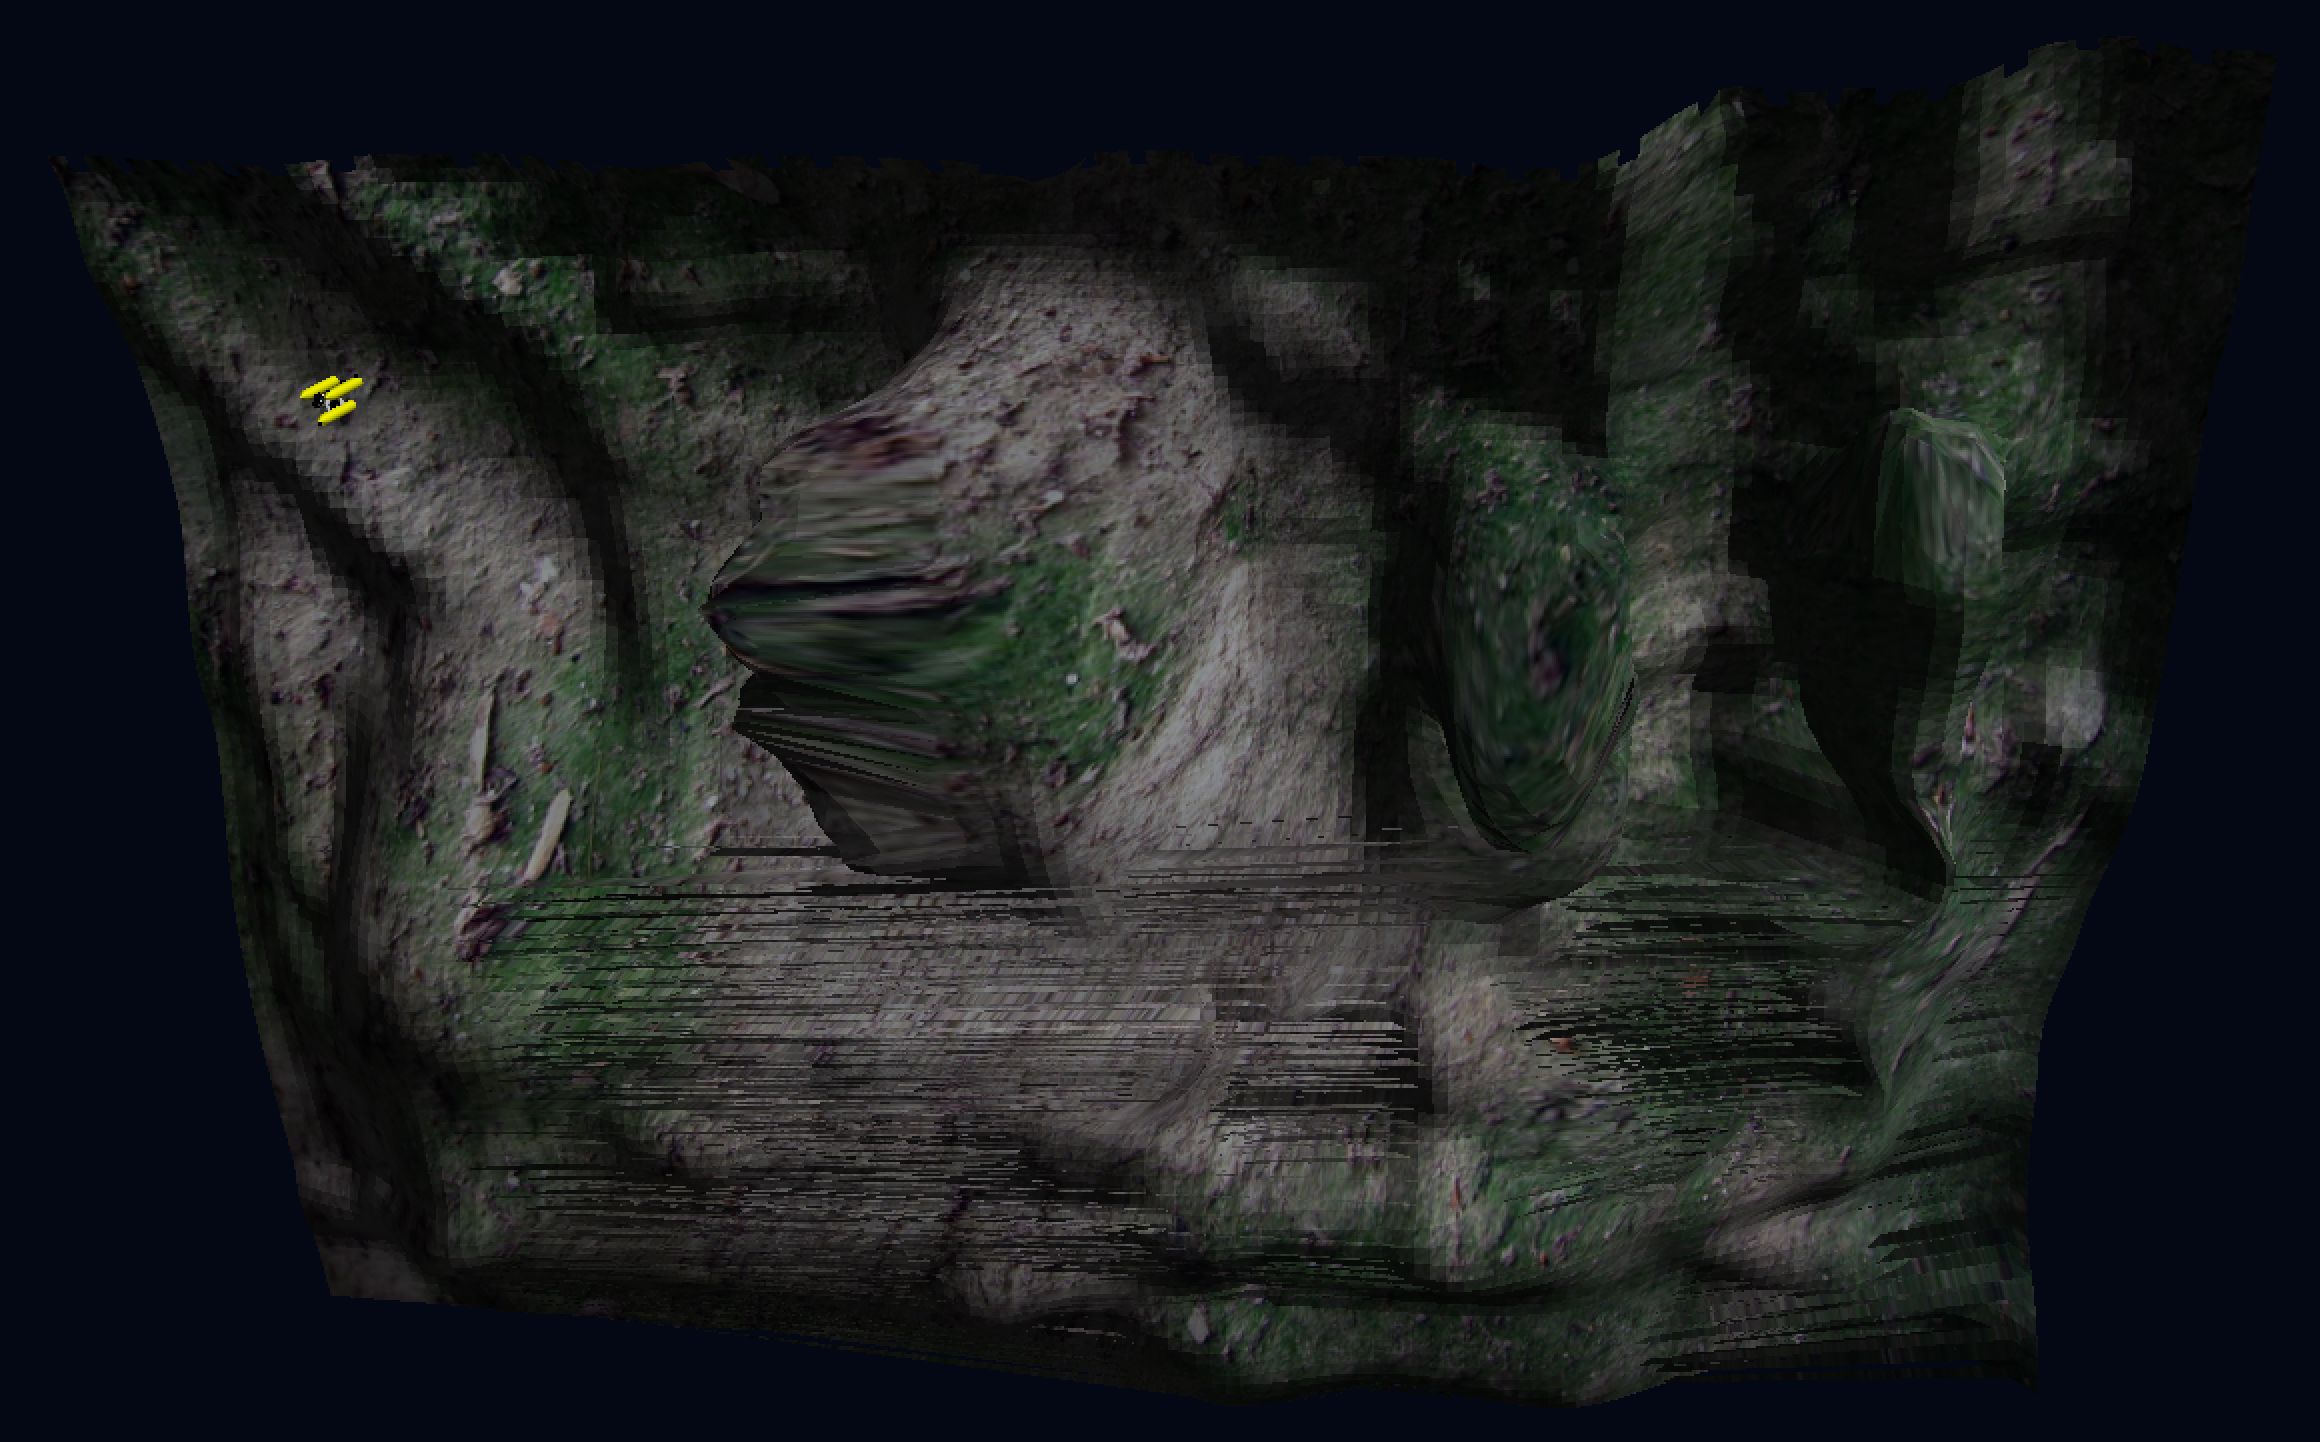
\includegraphics[width=0.48 \textwidth]{assets/reefOriginal}
    }
  \end{center}
\vspace{-20pt}
  \caption{Underwater Reef}
  \label{fig:reef}
\vspace{-10pt}
\end{wrapfigure}

We will be exploring the reef shown in \autoref{fig:reef} as a test. The idea of the basic algorithm that we will be using is shown in \autoref{fig:basicAlgorithm}. The robot starts in its starting position as shown in \autoref{fig:basicAlgorithm}. From there it will start scanning and move downwards until it either reaches the ground or a predefined \textit{maxDepth}. Once we reach that point the robot will move to the right for a predefined distance \textit{d}. At that point the robot goes back up until it reaches the predefined startDepth where it will go to the right for a predefined distance \textit{d}. This sequence is repeated until we reach the maxWidth.\\

\begin{wrapfigure}{c}{\textwidth}
\vspace{-26pt}
  \begin{center}
  \fbox{
    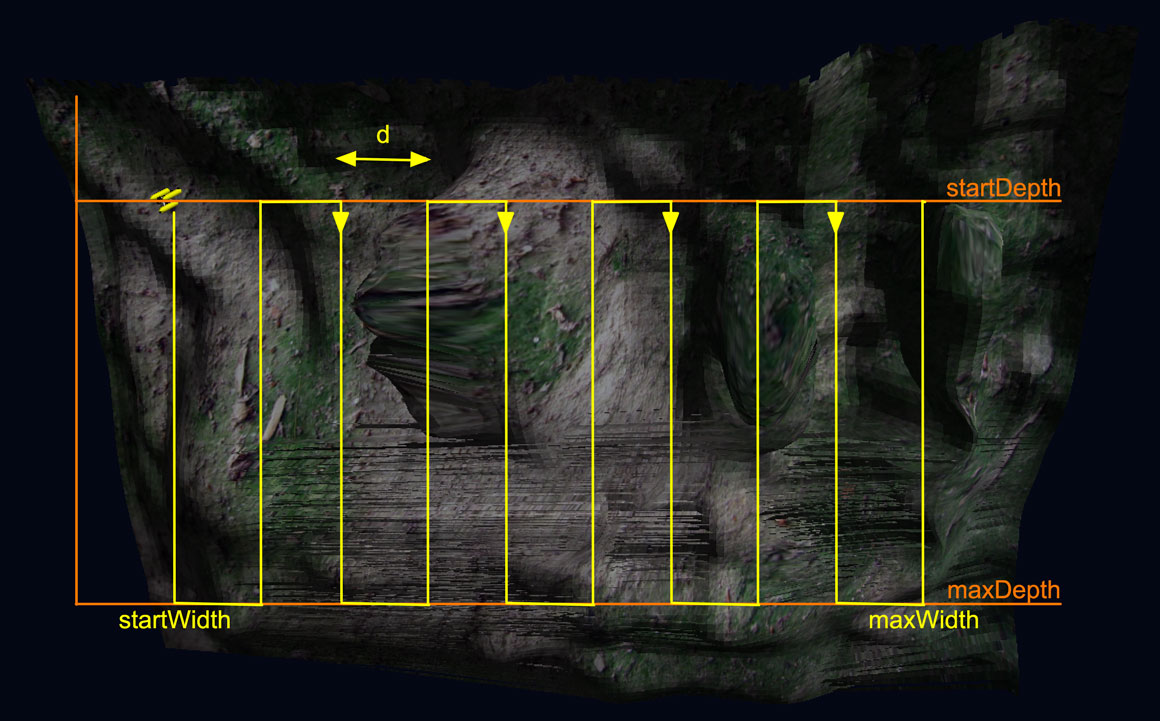
\includegraphics[width=0.90\textwidth]{assets/reefBasicAlgorithm.jpg}
    }
  \end{center}
\vspace{-20pt}
  \caption{Basic Algorithm}
  \label{fig:basicAlgorithm}
\end{wrapfigure}

\begin{wrapfigure}{l}{\textwidth}
\vspace{-50pt}
\end{wrapfigure}

Obviously the above algorithm only illustrates the basic idea. In reality, we have to also make sure the robot can actually move the way the algorithm wants it to move. Additionally, the robot should actually not be too far away from the reef so that it can scan the reef. In this paper we will therefore start from the basic algorithm discussed above and incrementally optimize until it successfully scans the reef. \\

\section{Related Work}
\label{sec:relatedworks}

The mapping of underwater structures is a common task in underwater robotics. Yet, only a few papers deal with the actual algorithm of mapping structures which is used to guide robots during their exploration. Therefore we could not find much previous work, especially none which deals with guidance algorithms for the mapping of a horizontal structure via an autonomous underwater robot.\\

One paper that deals with an actual guiding algorithm is \textit{A behavior-based architecture for autonomous underwater exploration} \cite{rosenblatt2002behavior}. There the authors use a behavior-based control architecture to safely guide a robot through a reef. Their robot follows a rope on the sea floor by utilizing a camera to get optical input. The rope acts as a tool for collision avoidance and path planning as it can be safely laid out by humans beforehand.\\

In another work, \textit{3-D terrain covering and map building algorithm for an AUV} \cite{lee20093}, the authors deal with the guidance and the mapping of an ocean floor with multiple islands or underwater mountains around. The approach they use is to explore the whole space by iteratively exploring a plane for each depth level. The situation and the approach used are drastically different from what we try to do as we try to scan horizontal structures and we do this using an improved interative approach.\\

There are many other papers that deal with cooperative exploration of multiple robots and the path planning for those robots. This does not apply well to our problem though, as we are only dealing with one robot and do not have to account for problems and challenges like the optimal division of work \cite{wu2012robust}. Most other papers which deal with actual guidance algorithms do so in combination with related mapping techniques like SLAM (e.g. \cite{makarenko2002experiment}).\\
  
\section{Preliminaries}
\label{sec:preliminaries}

\subsection{ROS \& Octomap}
For this research project we will make use of the Robot Operating System (ROS). ROS is a collection of frameworks for the development of robot control software. It provides us with many packages that implement functionalities like point cloud publishing and the simulation of different sensors. Within ROS, this project will use the octomap\_server \cite{hornung13auro}.\\

The octomap\_server works by listening to a 3D point cloud produced by one or more sensors and then combining those point cloud into an OctoMap. An OctoMap is a 3D map based on an underlying octree data structure. This OctoMap is then distributed to all nodes which are subscribed to the octomap server topics, in a compact binary format. Thus we can build and save 3D OctoMaps.\\

\subsection{Robot Overview}

The robot we will be using in this project has the following basic capabilities:
\begin{itemize}
\item movement along the x, y, and z axes,
\item rotation around the x, y, and z axes,
\item panning and tilting of sensor,
\item mapping functionality through range sensor,
\end{itemize}

Using these basic capabilities we are able to map sample reefs.

\begin{wrapfigure}{c}{\textwidth}
\vspace{-26pt}
  \begin{center}
  \fbox{
    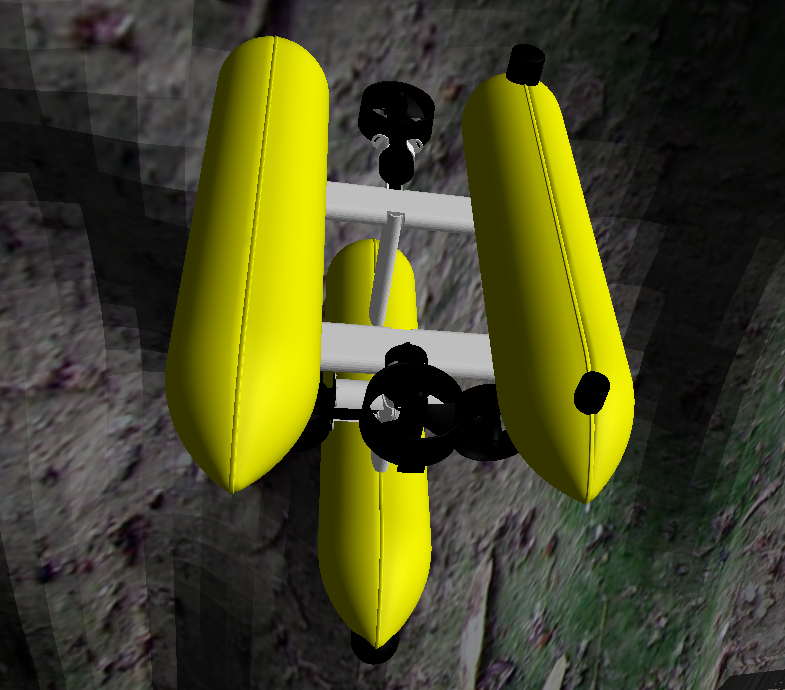
\includegraphics[width=0.70\textwidth]{assets/robot.png}
    }
  \end{center}
\vspace{-20pt}
  \caption{Basic Algorithm}
  \label{fig:basicAlgorithm}
\end{wrapfigure}

\begin{wrapfigure}{l}{\textwidth}
\vspace{-50pt}
\end{wrapfigure}

\newpage
\section{Towards an Optimal Scanning Algorithm}
\label{sec:optimalScanningAlgorithm}

Looking back to the initial idea of the algorithm which we illustrated in \autoref{sec:introduction}, we will now explore how to improve on this algorithm \cite{CoastLineExplorer:npentrel15}. First, we will ensure that the robot always keeps a minimum distance to the reef while also not being too far away from the reef.\\

\subsection{Distance Between Robot and Reef}
\label{sec:distanceBetweenRobotAndReef}
\begin{wrapfigure}{l}{0.27\textwidth}
\vspace{-28pt}
  \begin{center}
  \fbox{
    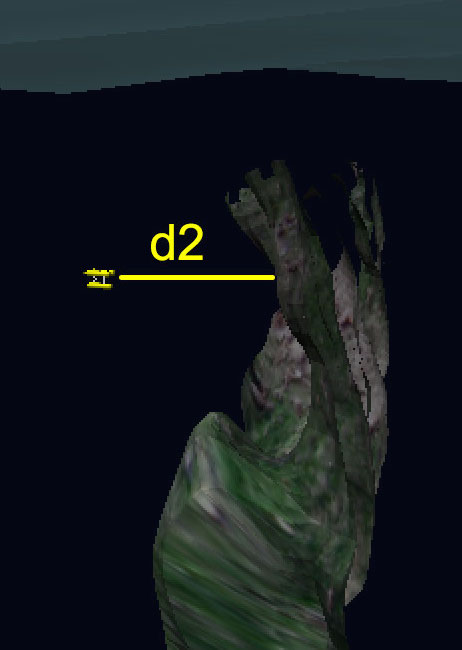
\includegraphics[width=0.25 \textwidth]{assets/reefSideways.jpg}
    }
  \end{center}
\vspace{-20pt}
  \caption{Reef Sideways}
  \label{fig:reef}
\vspace{20pt}
\end{wrapfigure}

If the robot starts in a random position, it is in our interest to get close enough to the reef to be able to scan the reef. Therefore we will move in the direction of the reef. To do this we use the following logic to check whether the robot is far enough away from the cliff to not crash but close enough to scan the cliff (see \autoref{fig:codeDistance}). Ideally the robot should always stay at exactly the \textit{minimumDistanceValue $\pm$ offset}. The \textit{scanDistance} is the scanned point of the reef that is closest to the robot.\\

\begin{wrapfigure}{c}{\textwidth}
\vspace{12pt}
\begin{lstlisting}[language=C++]
void ExploreAlgorithm::controlDistanceToCliff() {
    if(minimumDistanceValue > scanDistance) {
        moveTowardsCliff(); 
    } else if(minimumDistanceValue < (scanDistance - offset)) {
    	   moveAwayFromCliff();
    } 
}
\end{lstlisting} 
\vspace{-38pt}
  \caption{Pseudocode Snippet to Show how to Control the Distance to the Cliff}
  \label{fig:codeDistance}
  \vspace{20pt}
\end{wrapfigure}

\begin{wrapfigure}{l}{\textwidth}
\vspace{-50pt}
\end{wrapfigure}

The robot does not start to descend until it is within the specified distance away from the reef. Once it starts to descend it will continuously check if it is still within the specified distance. If this is not the case it will move horizontally either towards or away from the cliff to regain the specified distance using the logic illustrated in \autoref{fig:codeDistance}. When this is achieved it will continue its descend.\\

\begin{wrapfigure}{c}{\textwidth}
\vspace{0pt}
  \begin{center}
  \fbox{
    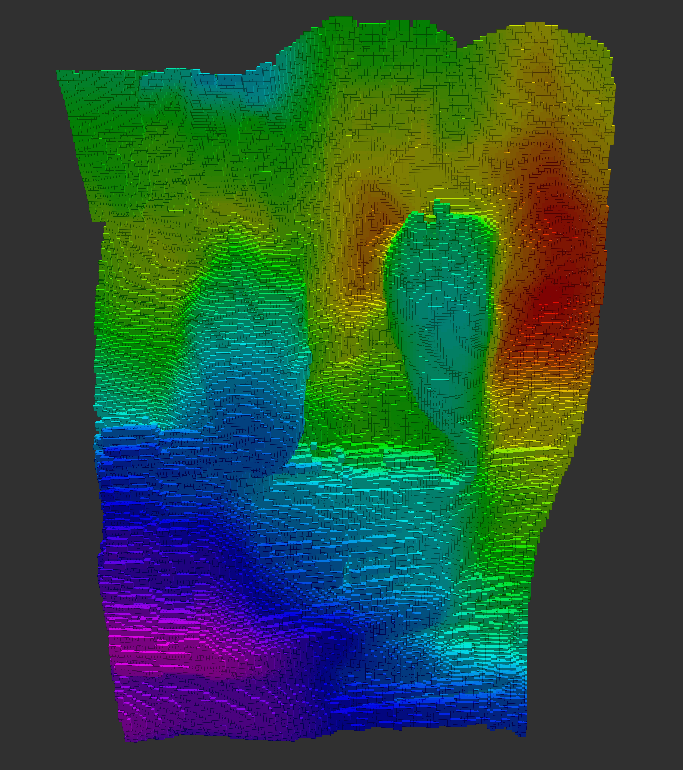
\includegraphics[width=0.47 \textwidth]{assets/MapOnlyDistance}
    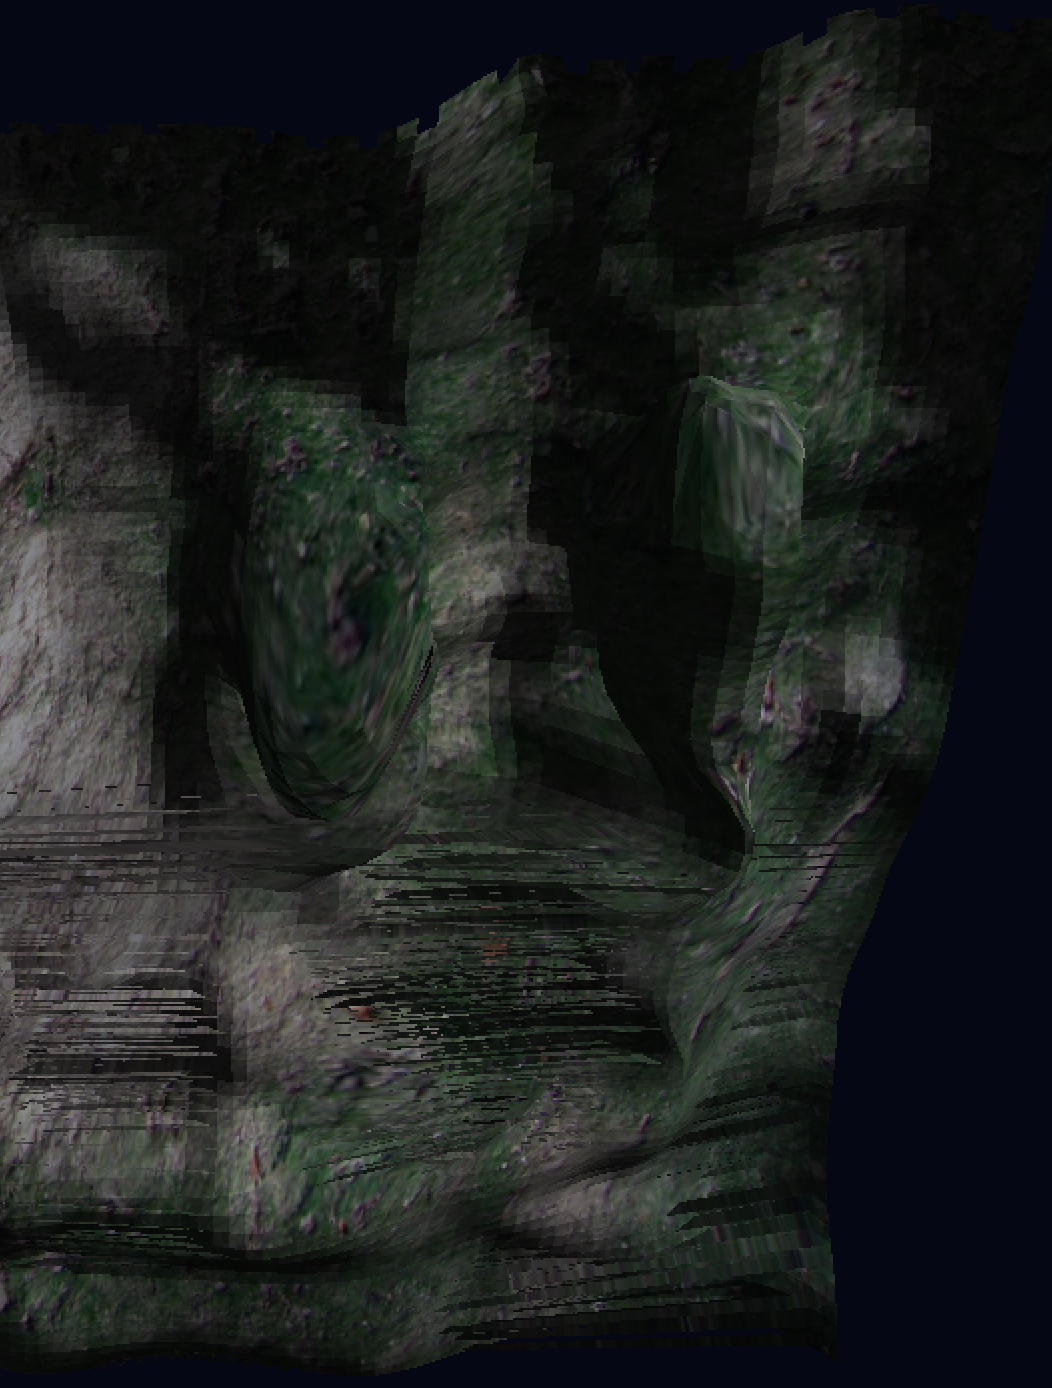
\includegraphics[width=0.4015 \textwidth]{assets/reefOriginalMappedComp}
    }
  \end{center}
\vspace{-20pt}
  \caption{Mapping using the Distance Algorithm}
  \label{fig:firstMapping}
\vspace{20pt}
\end{wrapfigure}

\begin{wrapfigure}{l}{\textwidth}
\vspace{-50pt}
\end{wrapfigure}

Overall this approach already provides us with good results as visible in \autoref{fig:firstMapping}. However, using this logic, the robot may run into issues because it does not have sensors above, below, or behind. This will not be covered in this paper but we will discuss this in \autoref{sec:limitations} and elaborate how it could be done in \autoref{sec:future}. Apart from running into objects, the robot can also fail to scan all areas due to the fact that we use the closest point in our field of vision to determine where we should be (see \autoref{fig:codeDistance}). In the case of spikes some areas may thus remain unscanned as can be seen in \autoref{fig:firstMappingProblems}. The latter problem will be discussed in the next subsection.\\

\begin{wrapfigure}{c}{\textwidth}
\vspace{-28pt}
  \begin{center}
  \fbox{
    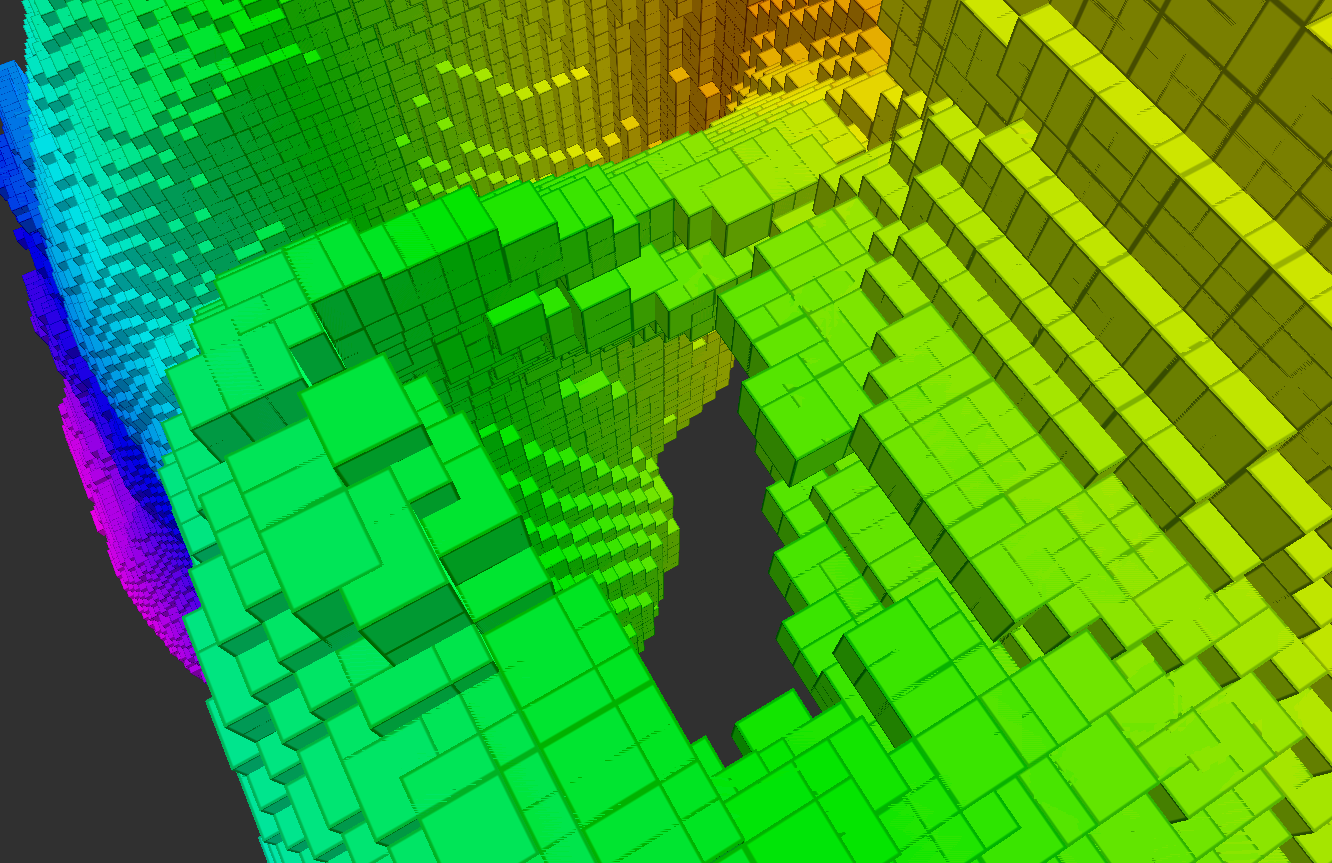
\includegraphics[width=0.23 \textwidth]{assets/MapOnlyDistanceHole1}
    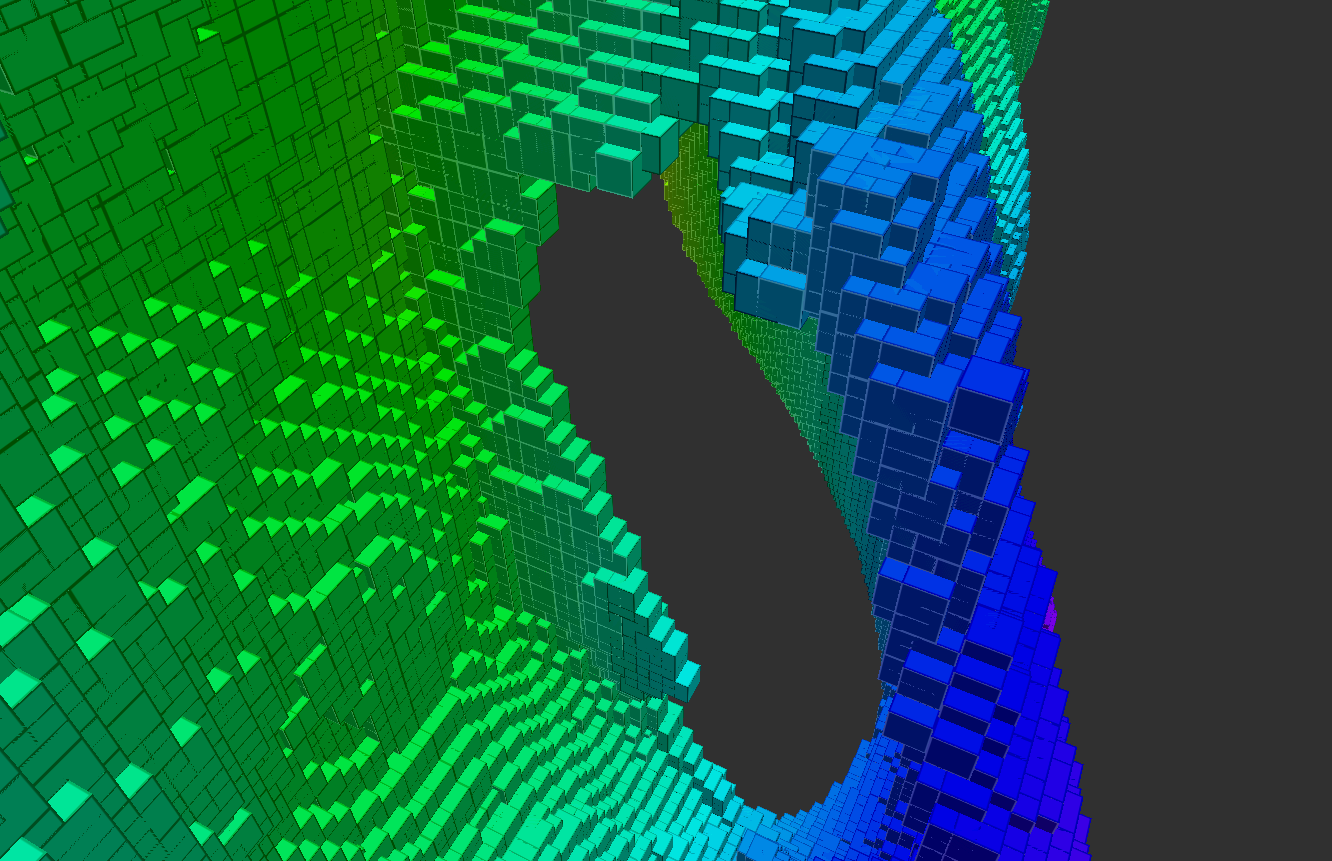
\includegraphics[width=0.23 \textwidth]{assets/MapOnlyDistanceHole2}
    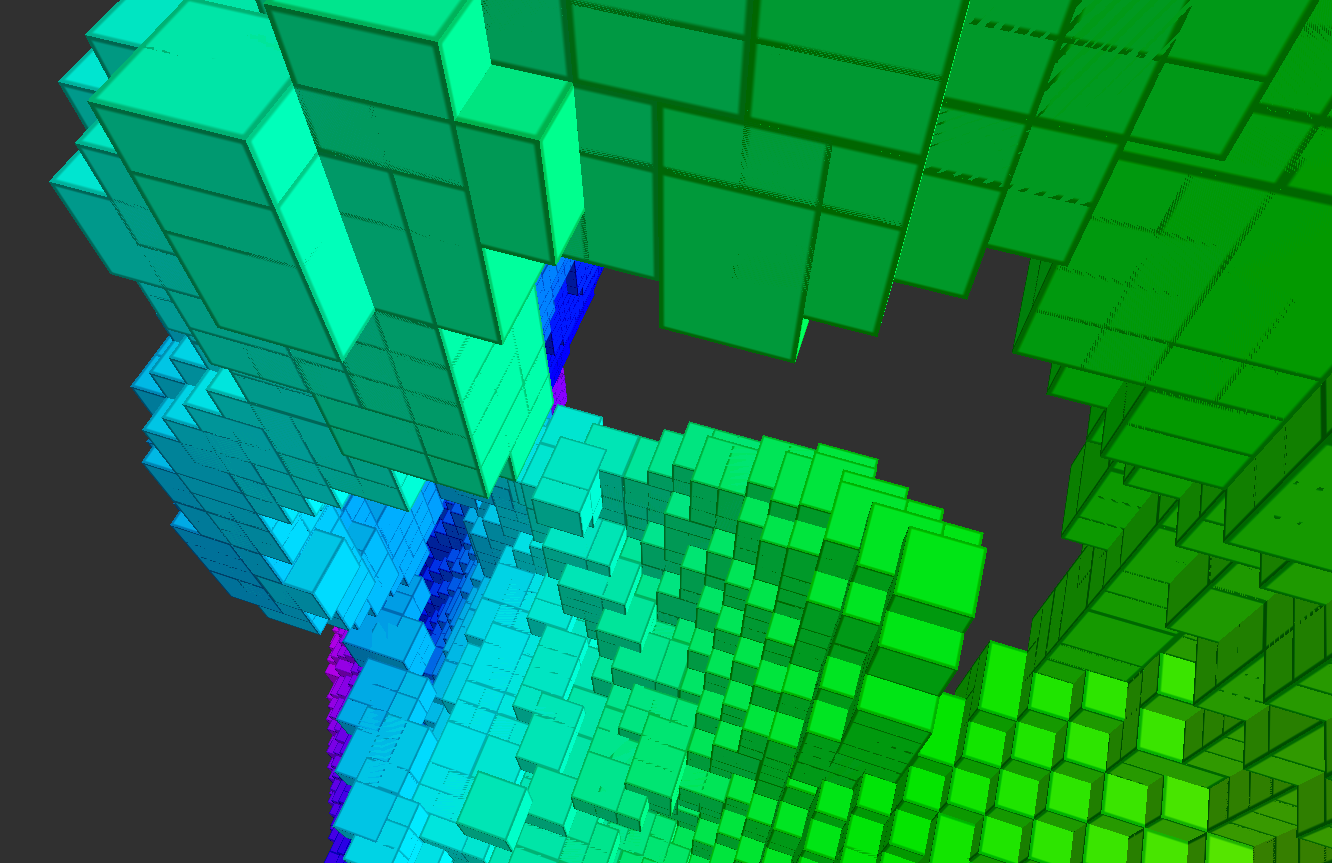
\includegraphics[width=0.23 \textwidth]{assets/MapOnlyDistanceHole3}
    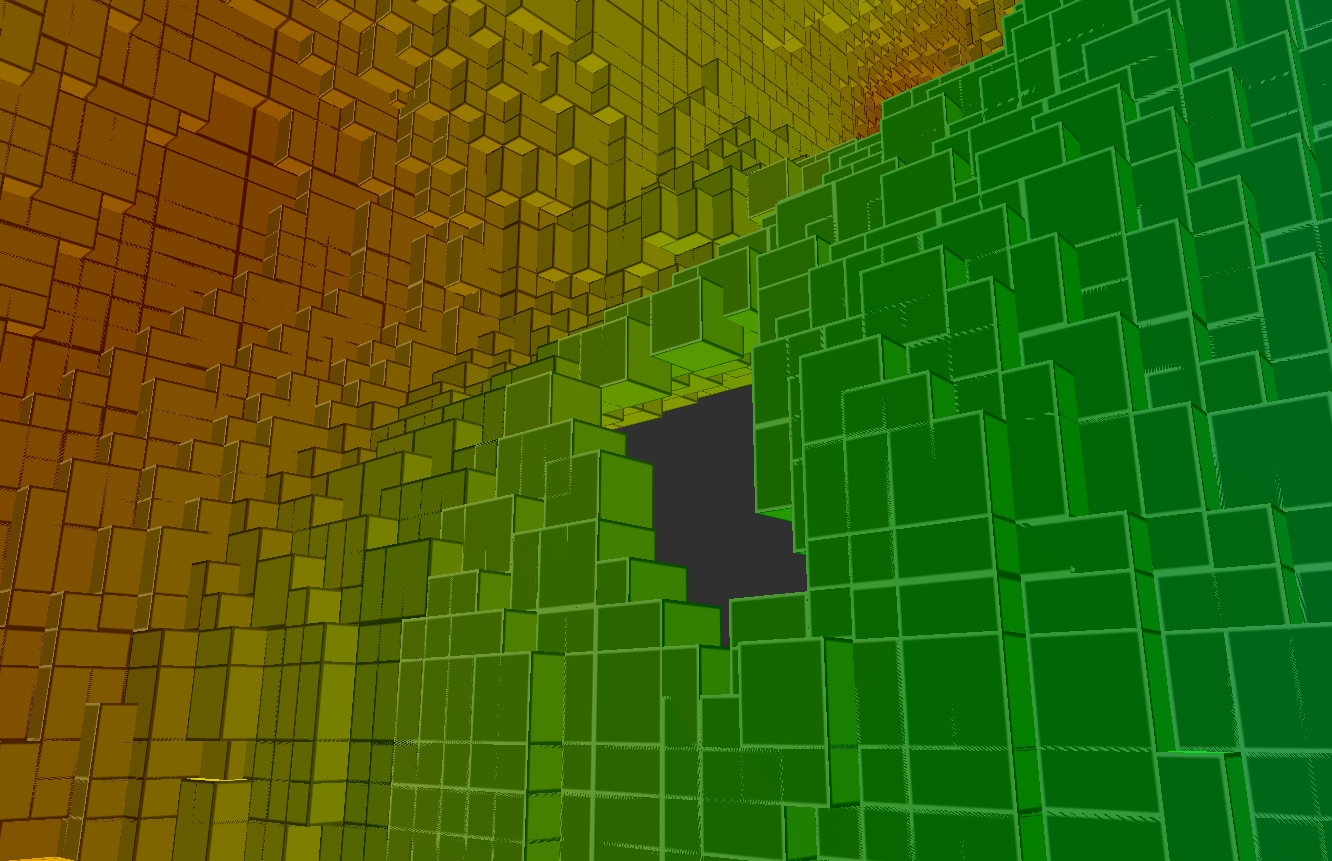
\includegraphics[width=0.23 \textwidth]{assets/MapOnlyDistanceHole4}
    }
  \end{center}
\vspace{-20pt}
  \caption{Mapping Problems using the Distance Algorithm}
  \label{fig:firstMappingProblems}
\vspace{20pt}
\end{wrapfigure}

\begin{wrapfigure}{l}{\textwidth}
\vspace{-50pt}
\end{wrapfigure}

\subsection{Improving the Value of scanDistance}
\label{sec:improvingValueOfScanDistance
}

In the previous section we have identified that one problem with our algorithm is that the value of \textit{scanDistance} might make us not explore areas because of spikes. While we need to make sure that the robot does not crash into anything, we still want to maximize what we can scan. Therefore, we will calculate the value \textit{scanDistance} not of the full field of vision of the robot but rather of a part of it that is as big as the robot.\\

\begin{wrapfigure}{l}{0.45\textwidth}
\vspace{-28pt}
  \begin{center}
  \fbox{
    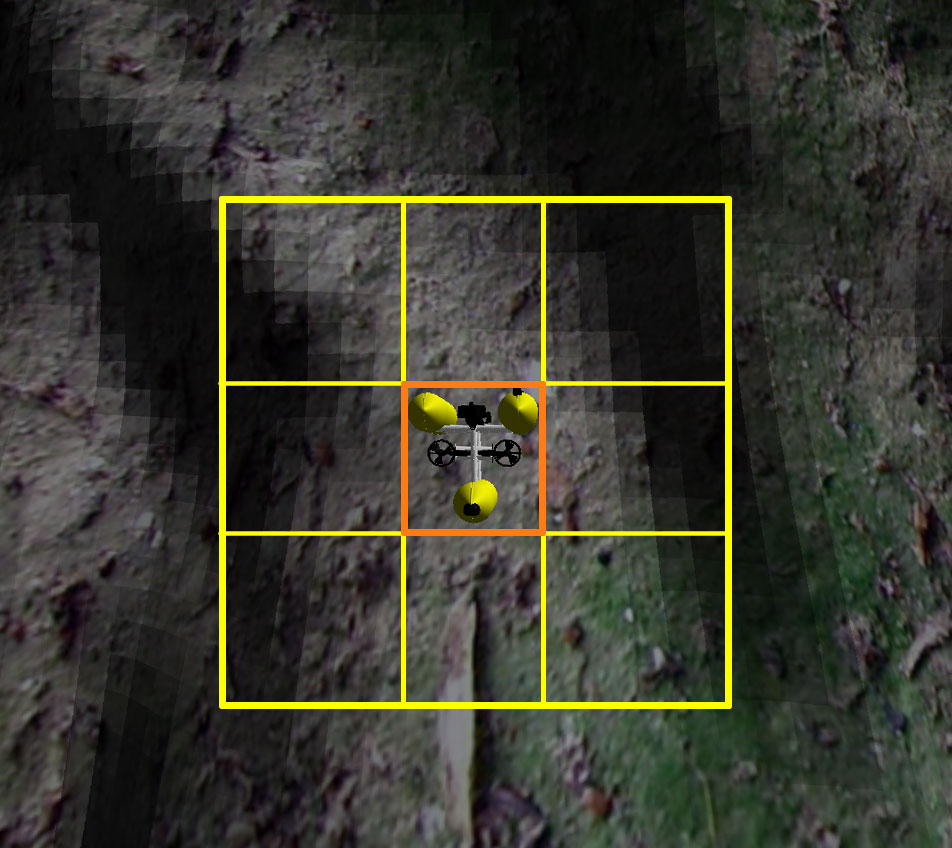
\includegraphics[width=0.42 \textwidth]{assets/ReducedDistanceExplain.jpg}
    }
  \end{center}
\vspace{-20pt}
  \caption{Robot's Field of Vision}
  \label{fig:reducedDistanceExplain}
\vspace{20pt}
\end{wrapfigure}

Using the subpart of the field of vision of the robot that is as big as the robot ensures that we can move as close as possible to the reef while still not crashing into anything. This is illustrated in \autoref{fig:reducedDistanceExplain}. In \autoref{sec:distanceBetweenRobotAndReef}, the robot would take the whole field of vision illustrated by the outer yellow rectangle. In the new approach we would like to only use the smaller orange rectangle.\\

\begin{wrapfigure}{c}{\textwidth}
\vspace{-2pt}
\begin{lstlisting}[language=C++]
double DistanceFinder::imageCb(const sensor_msgs::ImageConstPtr& msg) {
	cv_bridge::CvImageConstPtr cv_ptr = getImage(msg, msg->encoding);
	double scanDistance = std::numeric_limits<double>::max();
	int startRobotFieldWidth = (fieldOfVisionWidth - robotWidth)/2;
	int endRobotFieldWidth = startRobotField + robotWidth;
	int startRobotFieldHeight = (fieldOfVisionHeight - robotHeight)/2;
	int endRobotFieldHeight = startRobotFieldHeight + robotWidth;
	
	for(int i = startRobotFieldWidth; i < endRobotFieldWidth; i++)
		for(int j = startRobotFieldHeight; j < endRobotFieldHeight; j++)
			if(cv_ptr->image.at<float>(i,j) < scanDistance)
				scanDistance = cv_ptr->image.at<float>(i,j);
	return scanDistance;
}
\end{lstlisting} 
\vspace{-38pt}
  \caption{Pseudocode Snippet to Show how to Control the Distance to the Cliff}
  \label{fig:codeReducedDistance}
  \vspace{60pt}
\end{wrapfigure}

\begin{wrapfigure}{l}{\textwidth}
\vspace{-50pt}
\end{wrapfigure}

The code in \autoref{fig:codeReducedDistance} will return the correct \textit{scanDistance} for the area of the robot robotField. This value will now be used in the code which we use to keep the correct distance to the reef (see \autoref{fig:codeDistance}). Using this improved version of the algorithm, the newly scanned map is better. The overall scanned map can be see in \autoref{fig:secondMapping}.\\

\begin{wrapfigure}{c}{\textwidth}
\vspace{0pt}
  \begin{center}
  \fbox{
    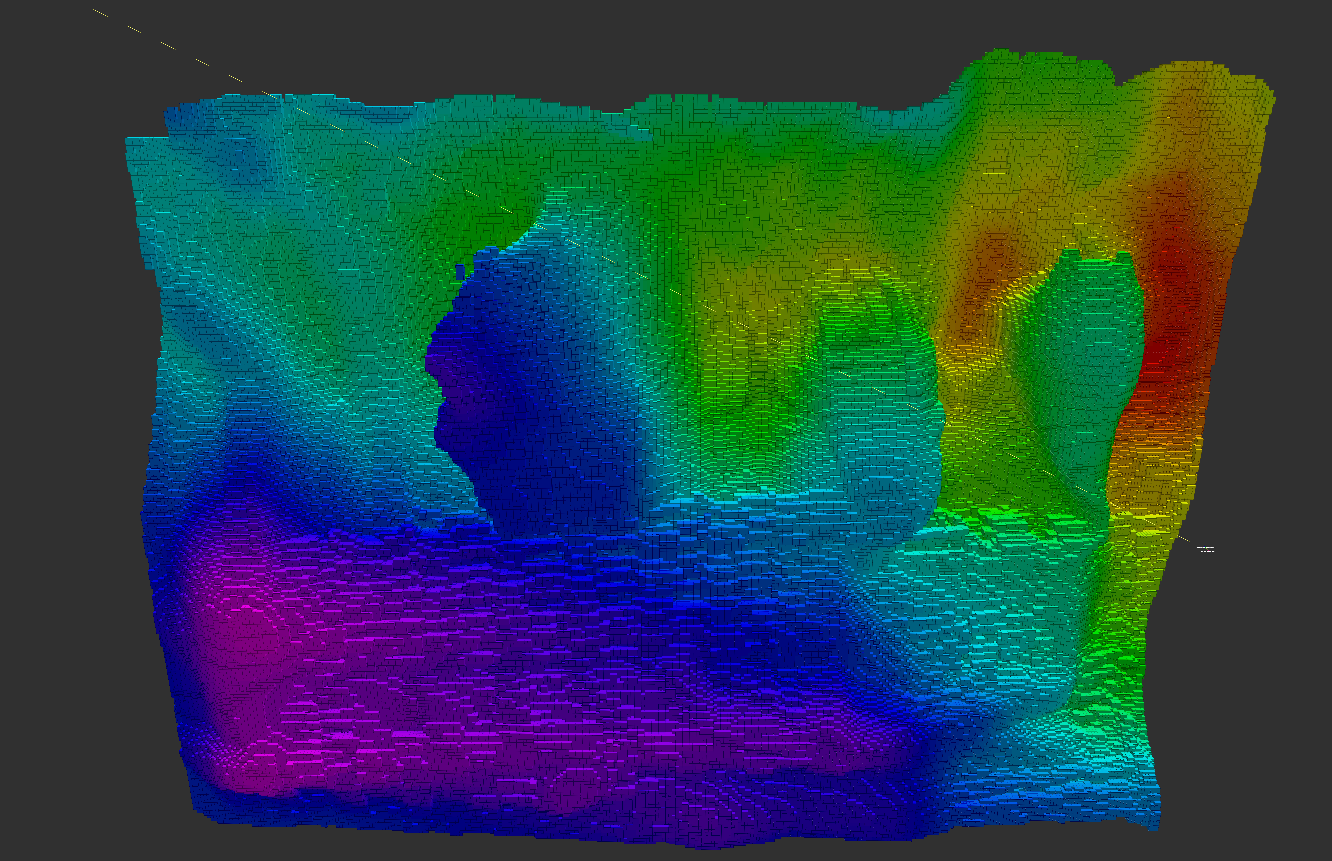
\includegraphics[width=0.47 \textwidth]{assets/ReducedDistanceFinding}
    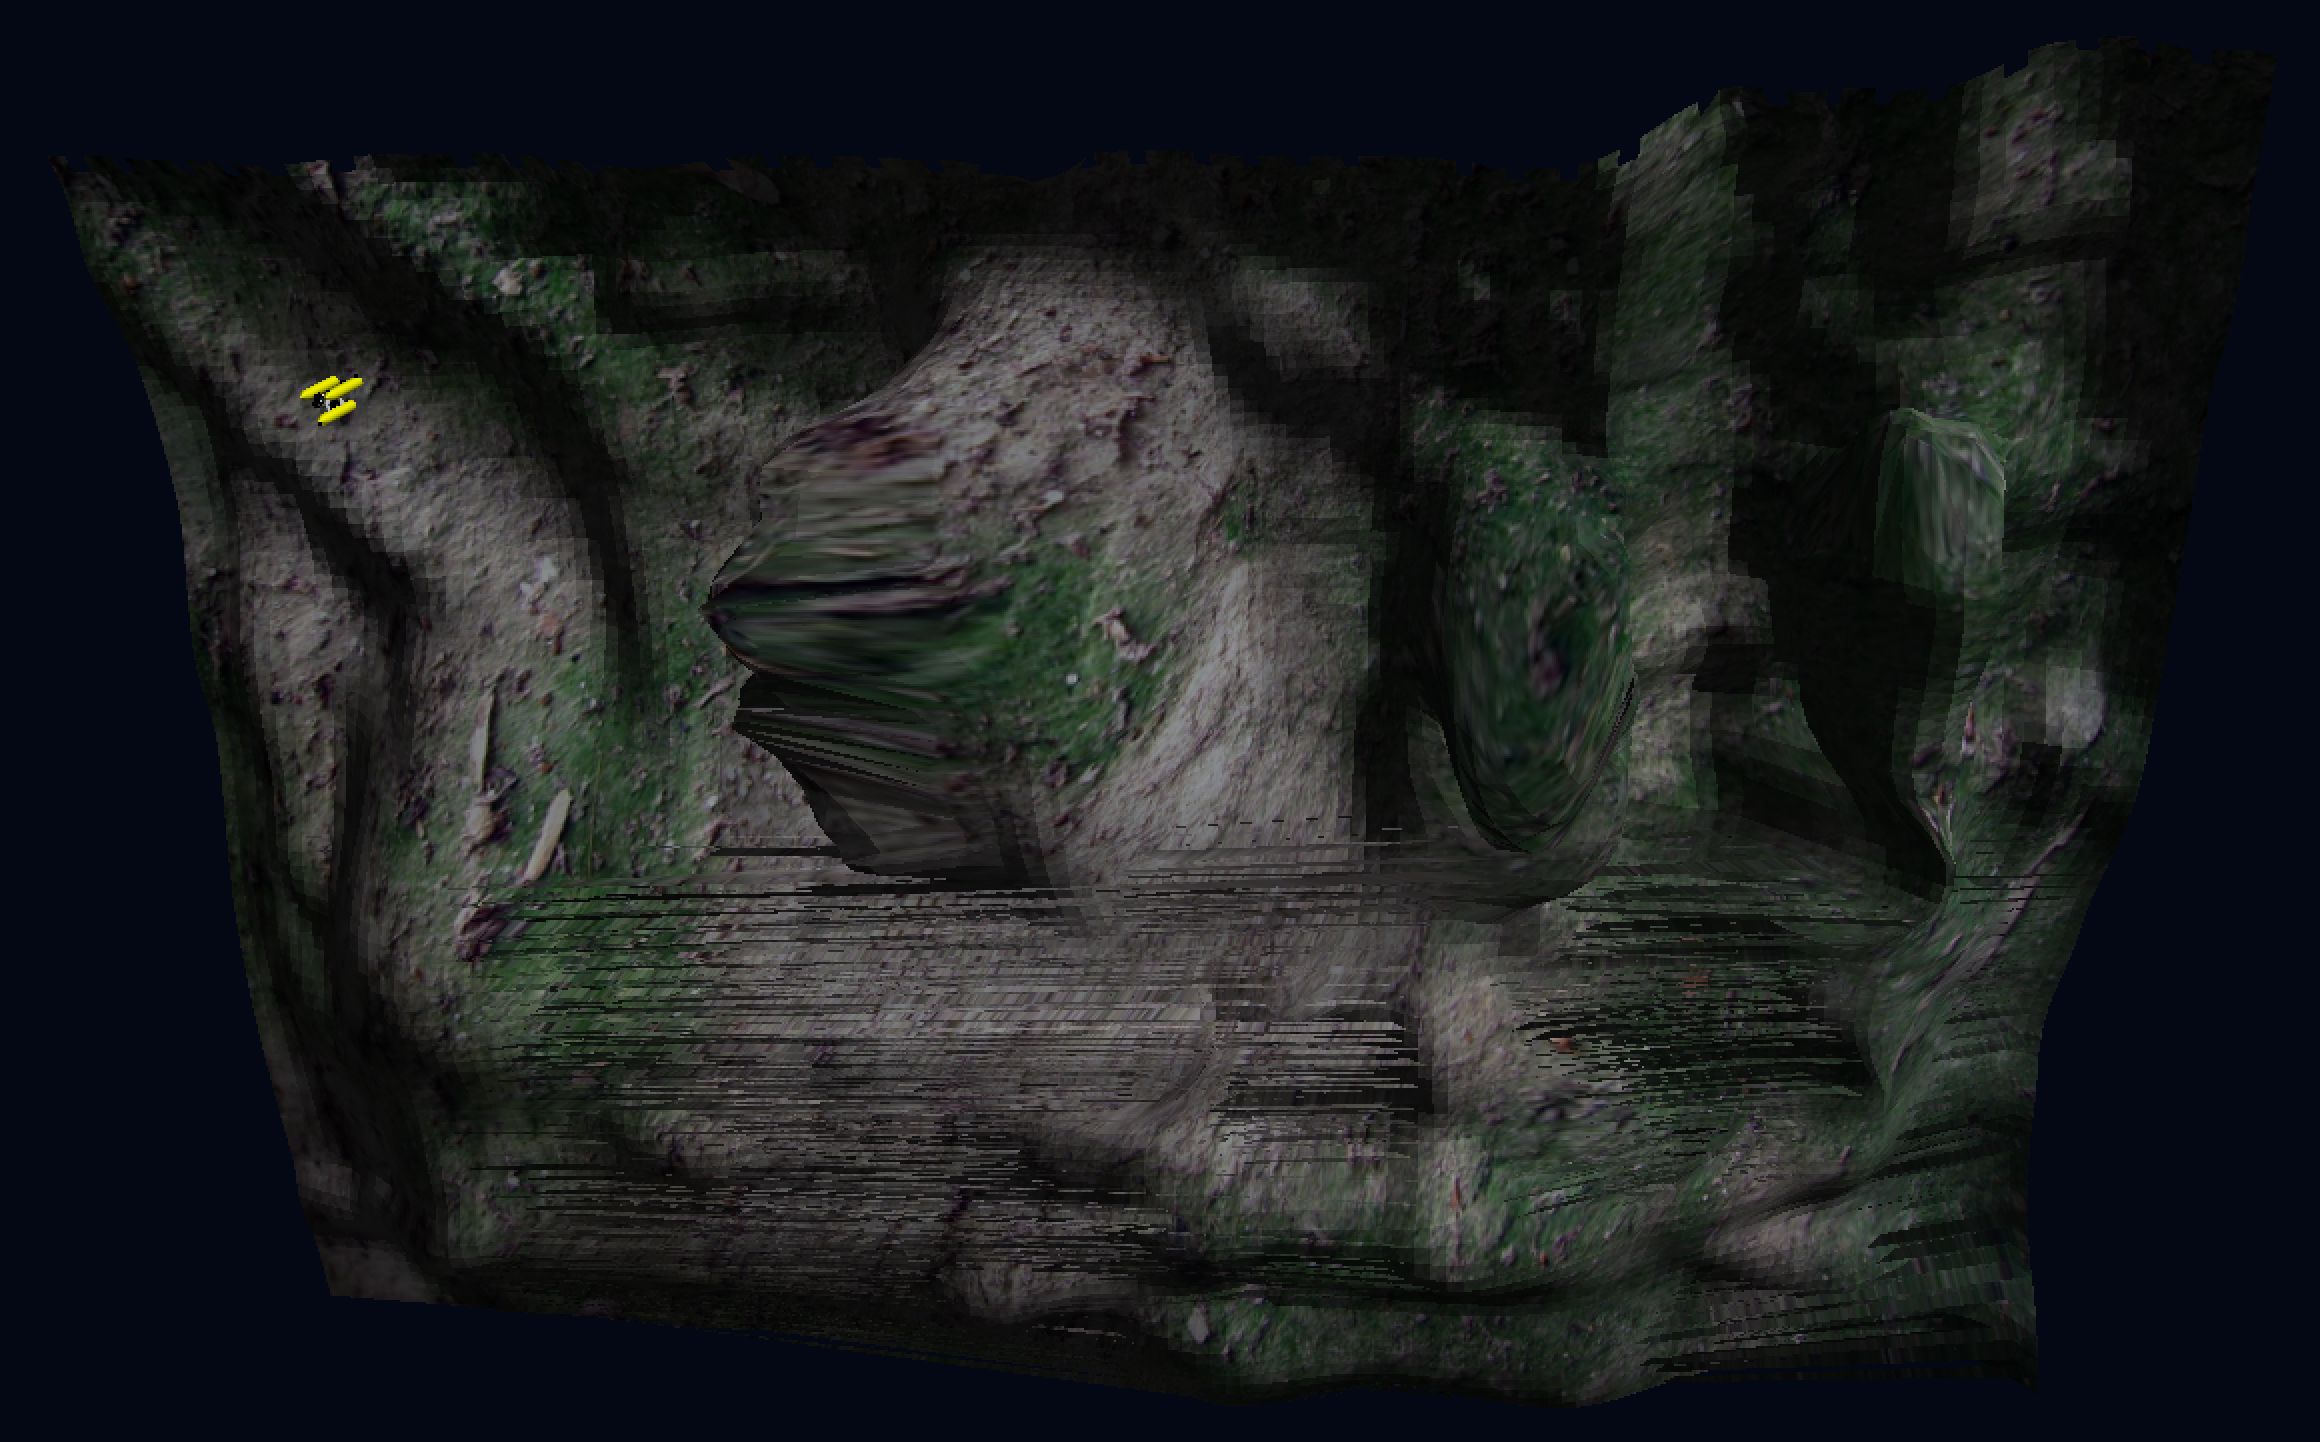
\includegraphics[width=0.49 \textwidth]{assets/reefOriginal}
    }
  \end{center}
\vspace{-20pt}
  \caption{Mapping using the Distance Algorithm}
  \label{fig:secondMapping}
\vspace{20pt}
\end{wrapfigure}

\begin{wrapfigure}{l}{\textwidth}
\vspace{-50pt}
\end{wrapfigure}

When examining the map closer, we again look for holes in the map. Specifically, we will again look at the places where we found holes in the map before (see \autoref{fig:firstMappingProblems}). As can be seen in \autoref{fig:secondMappingProblems}, one hole is completely gone. The three other holes are slightly reduced but not yet fully mapped. We will tackle them in the next section.\\

\begin{wrapfigure}{c}{\textwidth}
\vspace{-28pt}
  \begin{center}
  \fbox{
    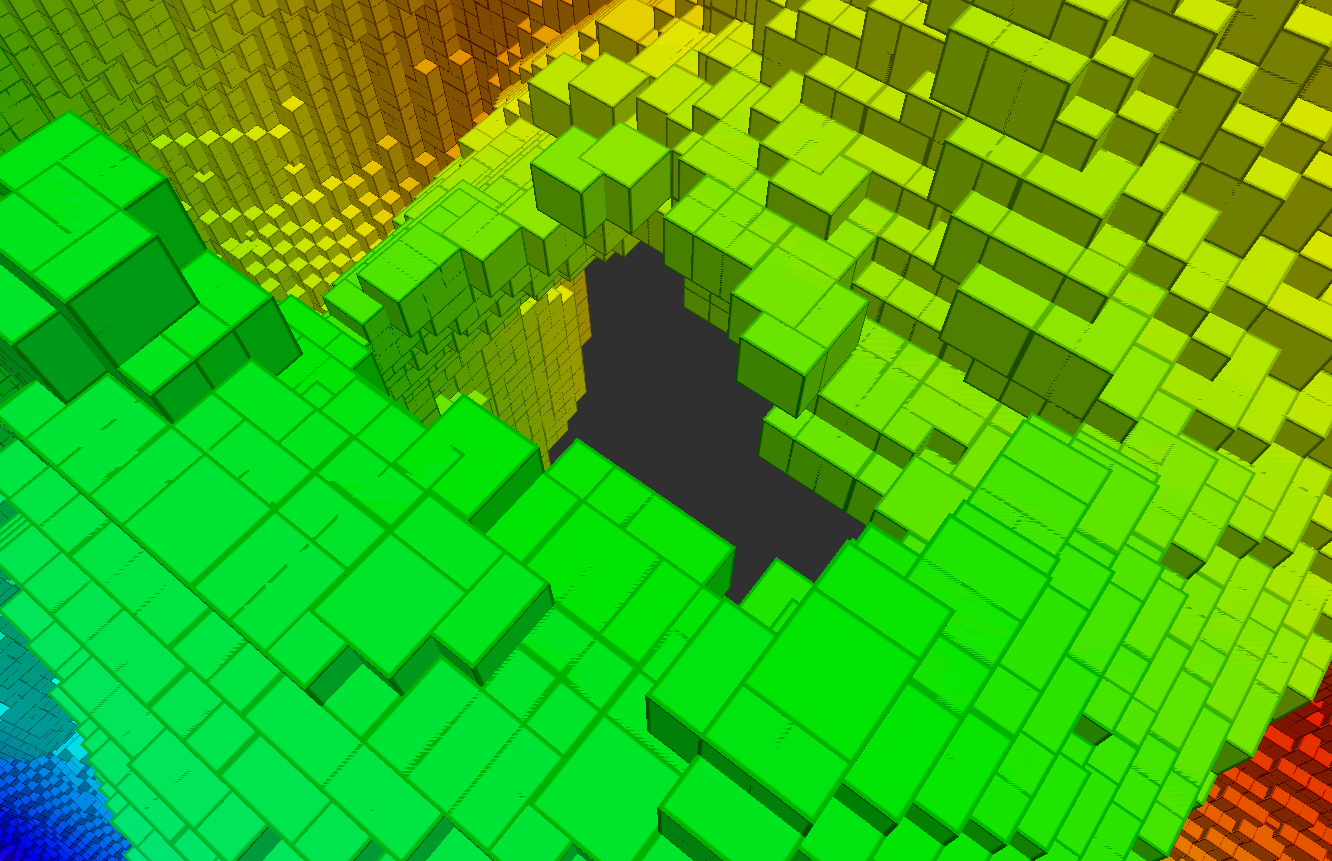
\includegraphics[width=0.23 \textwidth]{assets/ReducedDistanceFindingHole1}
    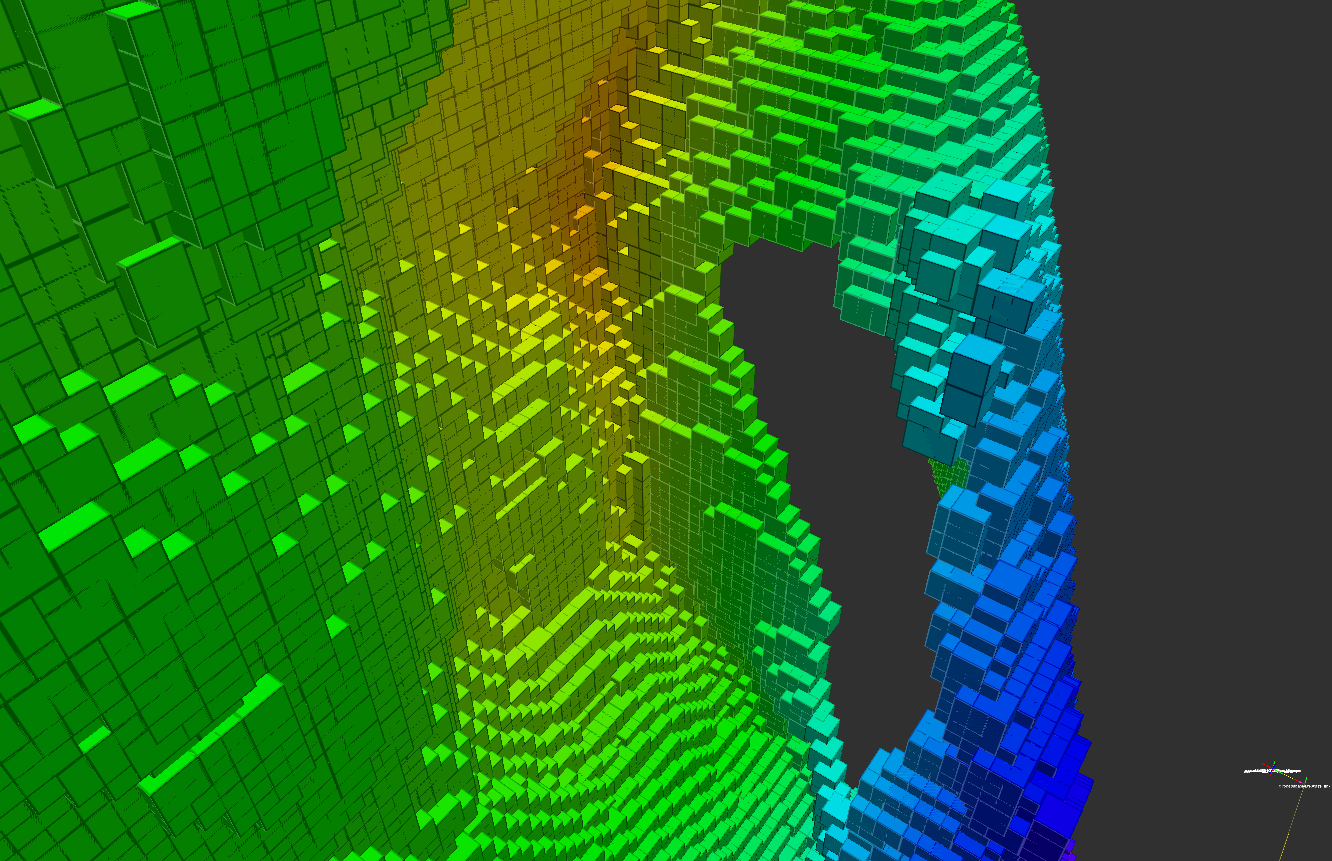
\includegraphics[width=0.23 \textwidth]{assets/ReducedDistanceFindingHole2}
    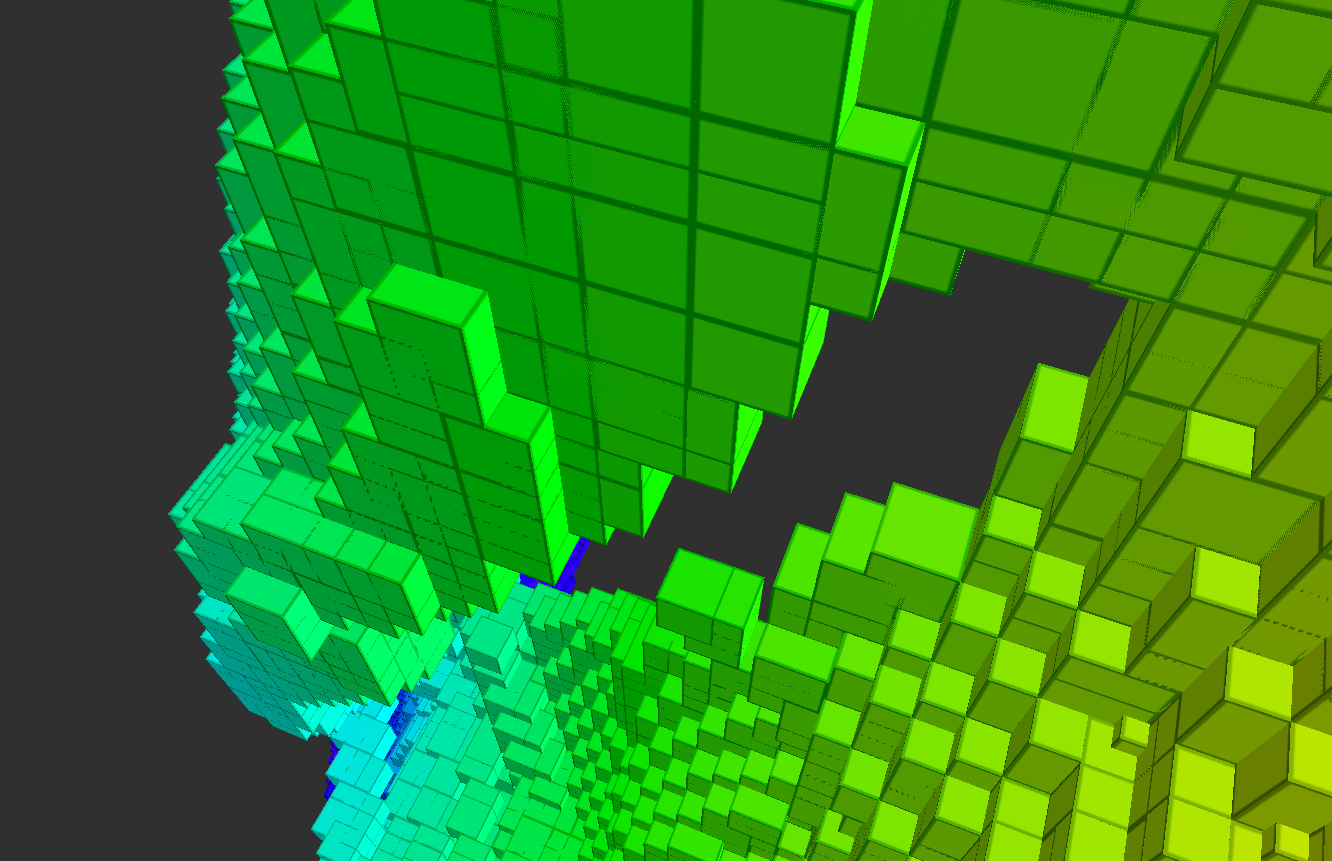
\includegraphics[width=0.23 \textwidth]{assets/ReducedDistanceFindingHole3}
    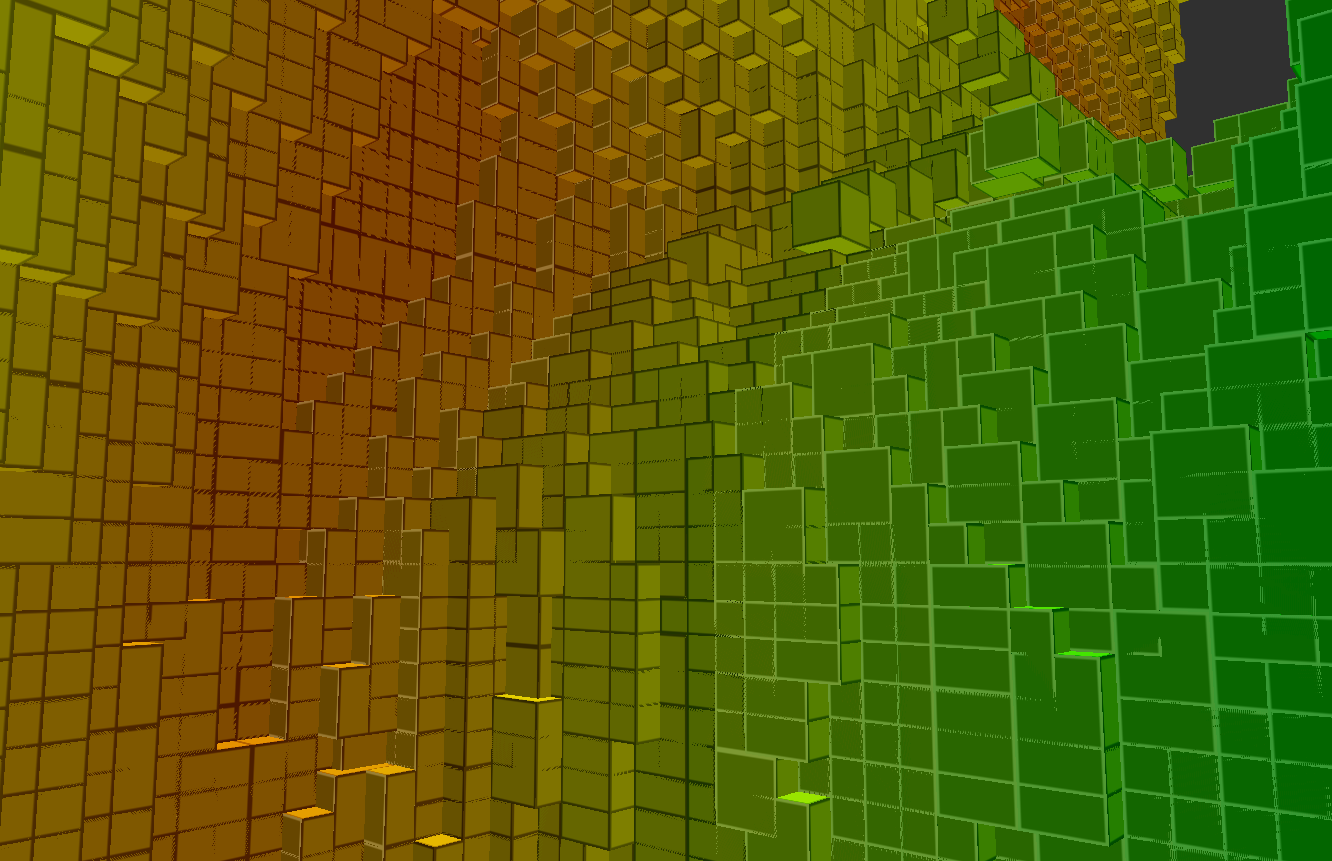
\includegraphics[width=0.23 \textwidth]{assets/ReducedDistanceFindingHole4}
    }
  \end{center}
\vspace{-20pt}
  \caption{Mapping Problems using the Distance Algorithm}
  \label{fig:secondMappingProblems}
\vspace{20pt}
\end{wrapfigure}

\begin{wrapfigure}{l}{\textwidth}
\vspace{-50pt}
\end{wrapfigure}

\subsection{Rotations}
The remaining holes are mostly on the sides of reef structures. Therefore we want to rotate our robot every few seconds around the z axis. Thus we scan the sides of the reef structures as well. The approach we use could also be mimicked by moving the sensor but we chose to rotate the whole robot as can be seen in the code in \autoref{fig:codeRotation}.\\

\begin{wrapfigure}{c}{\textwidth}
\vspace{-2pt}
\begin{lstlisting}[language=C++]
void ExploreAlgorithm::rotateAround() {
    tf::Quaternion q = this->transform.getRotation();
    tf::Matrix3x3 m(q);
    this->odom.twist.twist.angular.z = 1;
    double yaw = getCurrentYaw(m) 
    yaw = yaw + PI;
    if (fullyRotated(yaw)) {
		stopRotating();
    }
    this->position_pub.publish(this->odom);
}
\end{lstlisting} 
\vspace{-38pt}
  \caption{Pseudocode Snippet to Show how to Control the Distance to the Cliff}
  \label{fig:codeRotation}
  \vspace{22pt}
\end{wrapfigure}

\begin{wrapfigure}{l}{\textwidth}
\vspace{-100pt}
\end{wrapfigure}

The code turns the robot 360 degrees, hence once around its z-axis. This ensures that the sides of the reef structures are scanned as well. As can be seen in \autoref{fig:finalMapping}, this creates a full mapping of the area. When looking at the places where we previously had holes (see \autoref{fig:secondMappingProblems}), we notice that only one hole is still present. We have therefore successfully covered the other two. The remaining hole could be removed if we were to change the pitch of our robot.\footnote{To see a condensed video of the mapping see \href{http://youtu.be/LIdYnKuljzE}{http://youtu.be/LIdYnKuljzE}}\\

\begin{wrapfigure}{c}{\textwidth}
\vspace{-20pt}
  \begin{center}
  \fbox{
    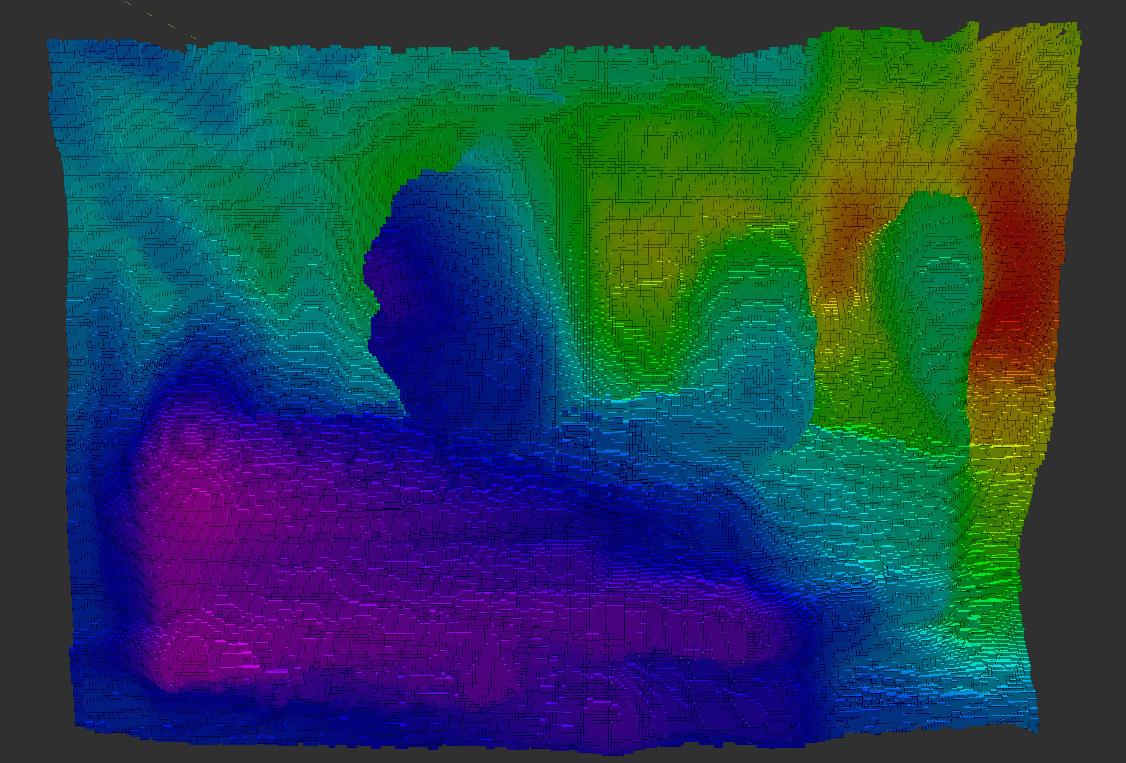
\includegraphics[width=0.45 \textwidth]{assets/FinalMapping}
    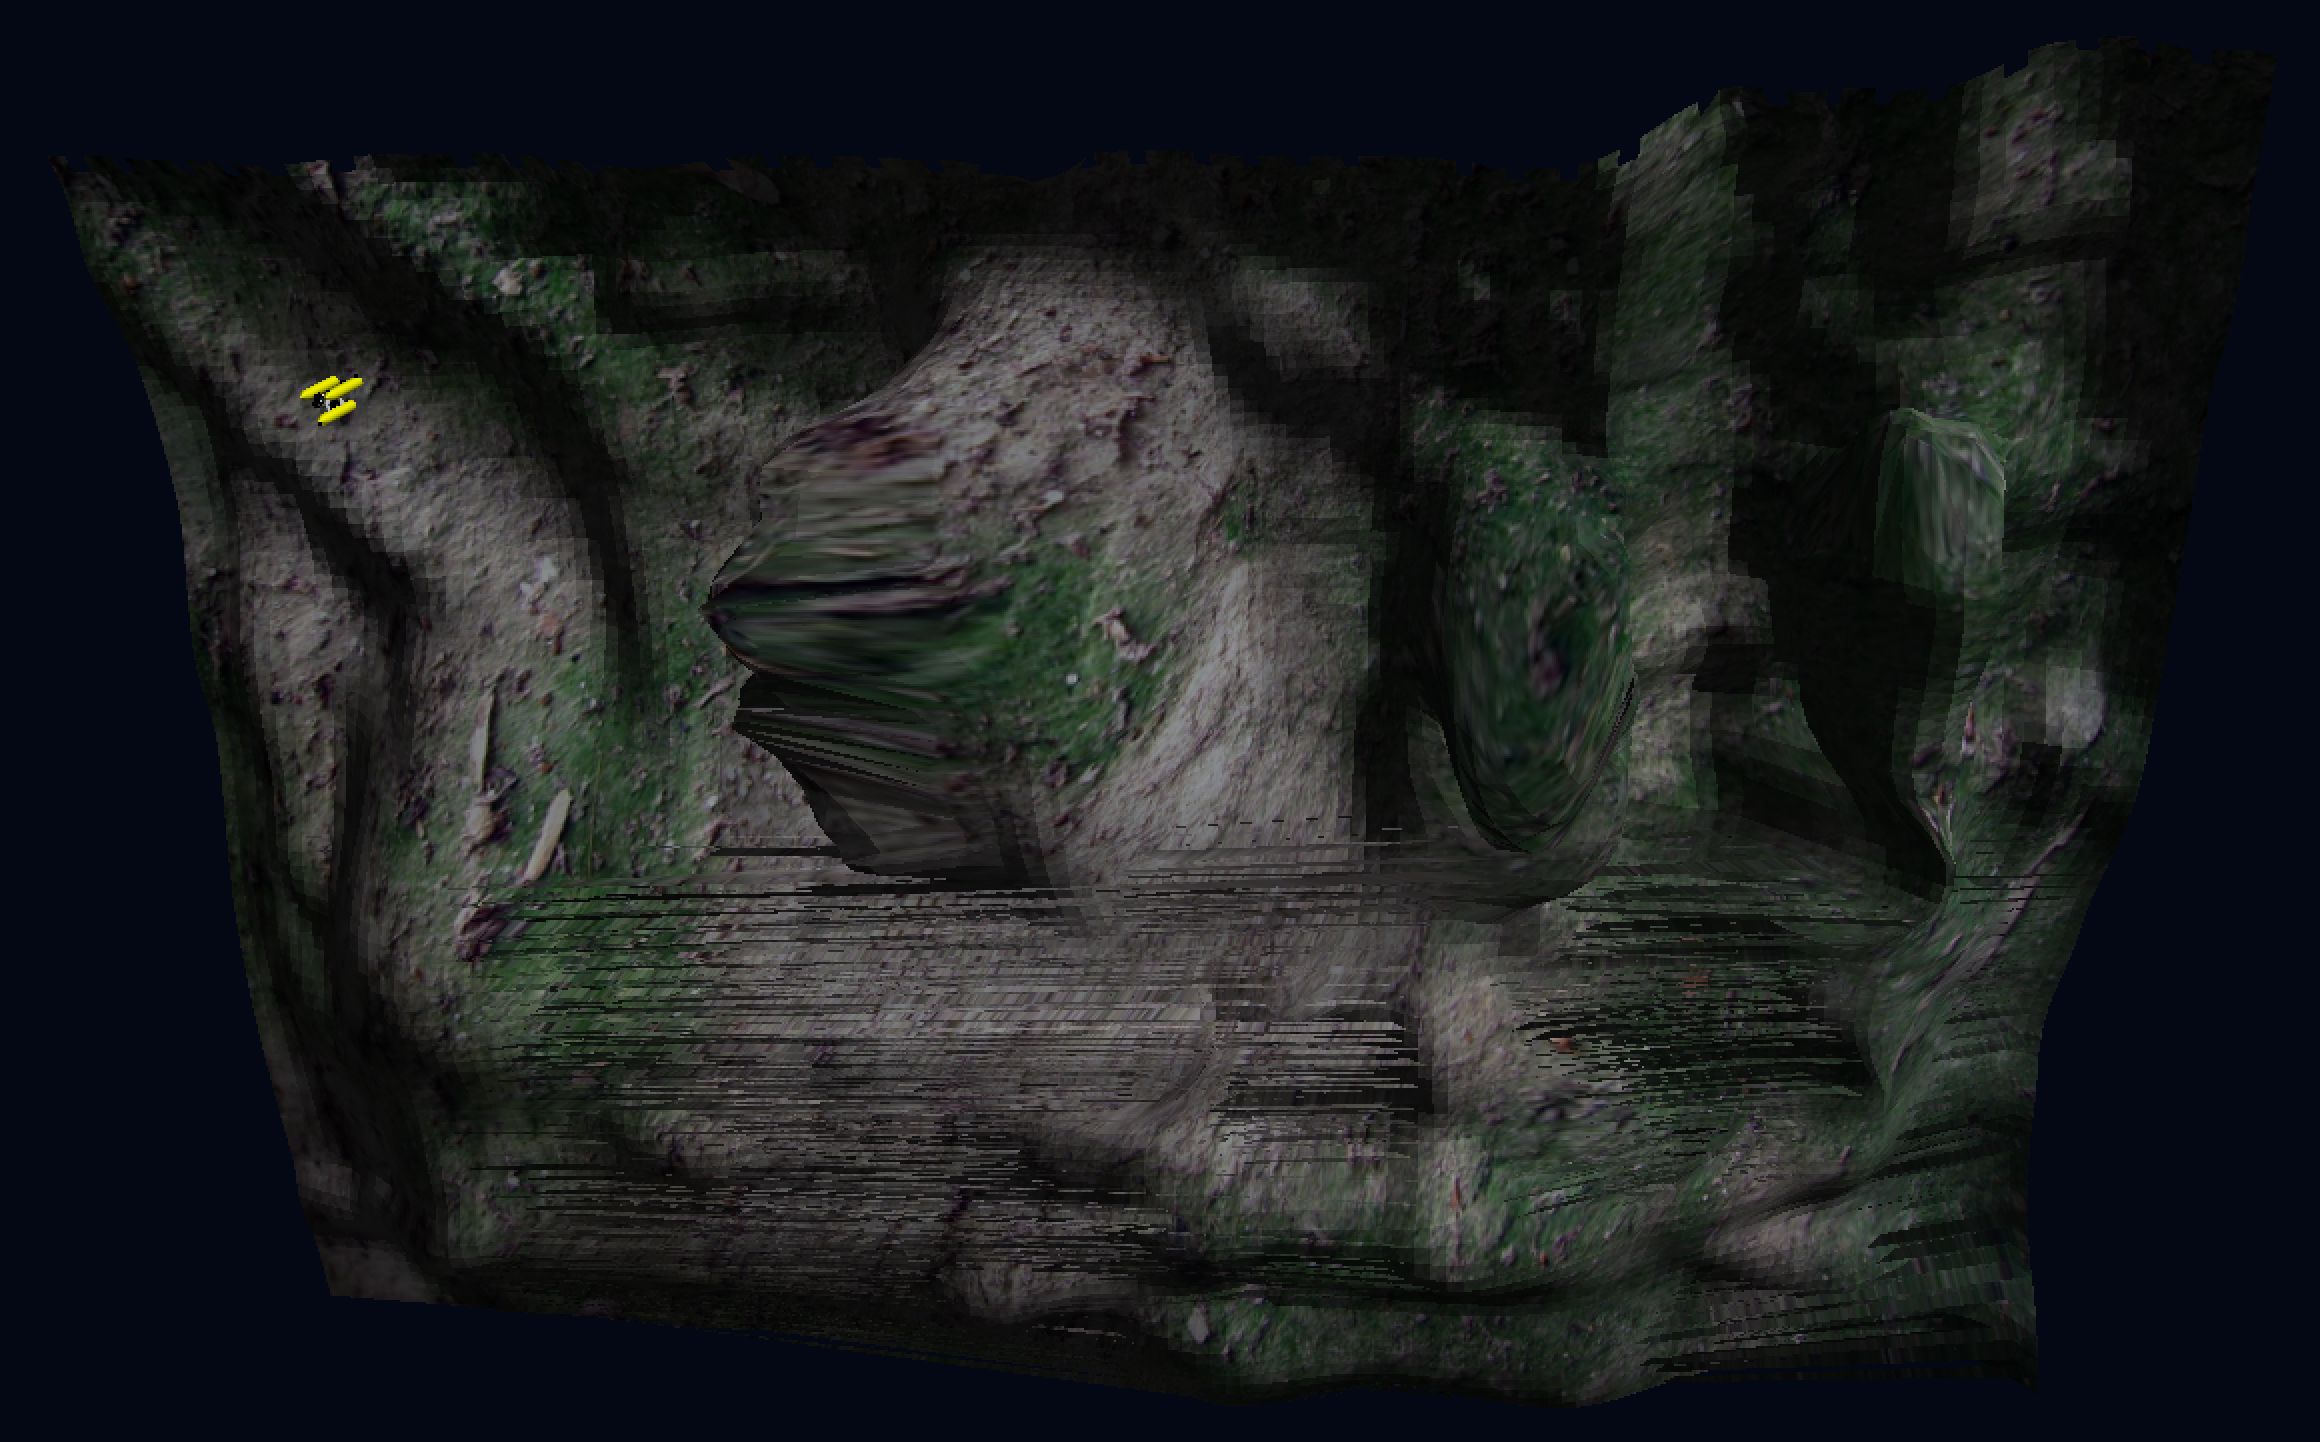
\includegraphics[width=0.49 \textwidth]{assets/reefOriginal}
    }
  \end{center}
\vspace{-20pt}
  \caption{Mapping using the Distance Algorithm with Rotation}
  \label{fig:finalMapping}
\vspace{12pt}
\end{wrapfigure}

\begin{wrapfigure}{l}{\textwidth}
\vspace{-100pt}
\end{wrapfigure}

\begin{wrapfigure}{c}{\textwidth}
\vspace{-28pt}
  \begin{center}
  \fbox{
    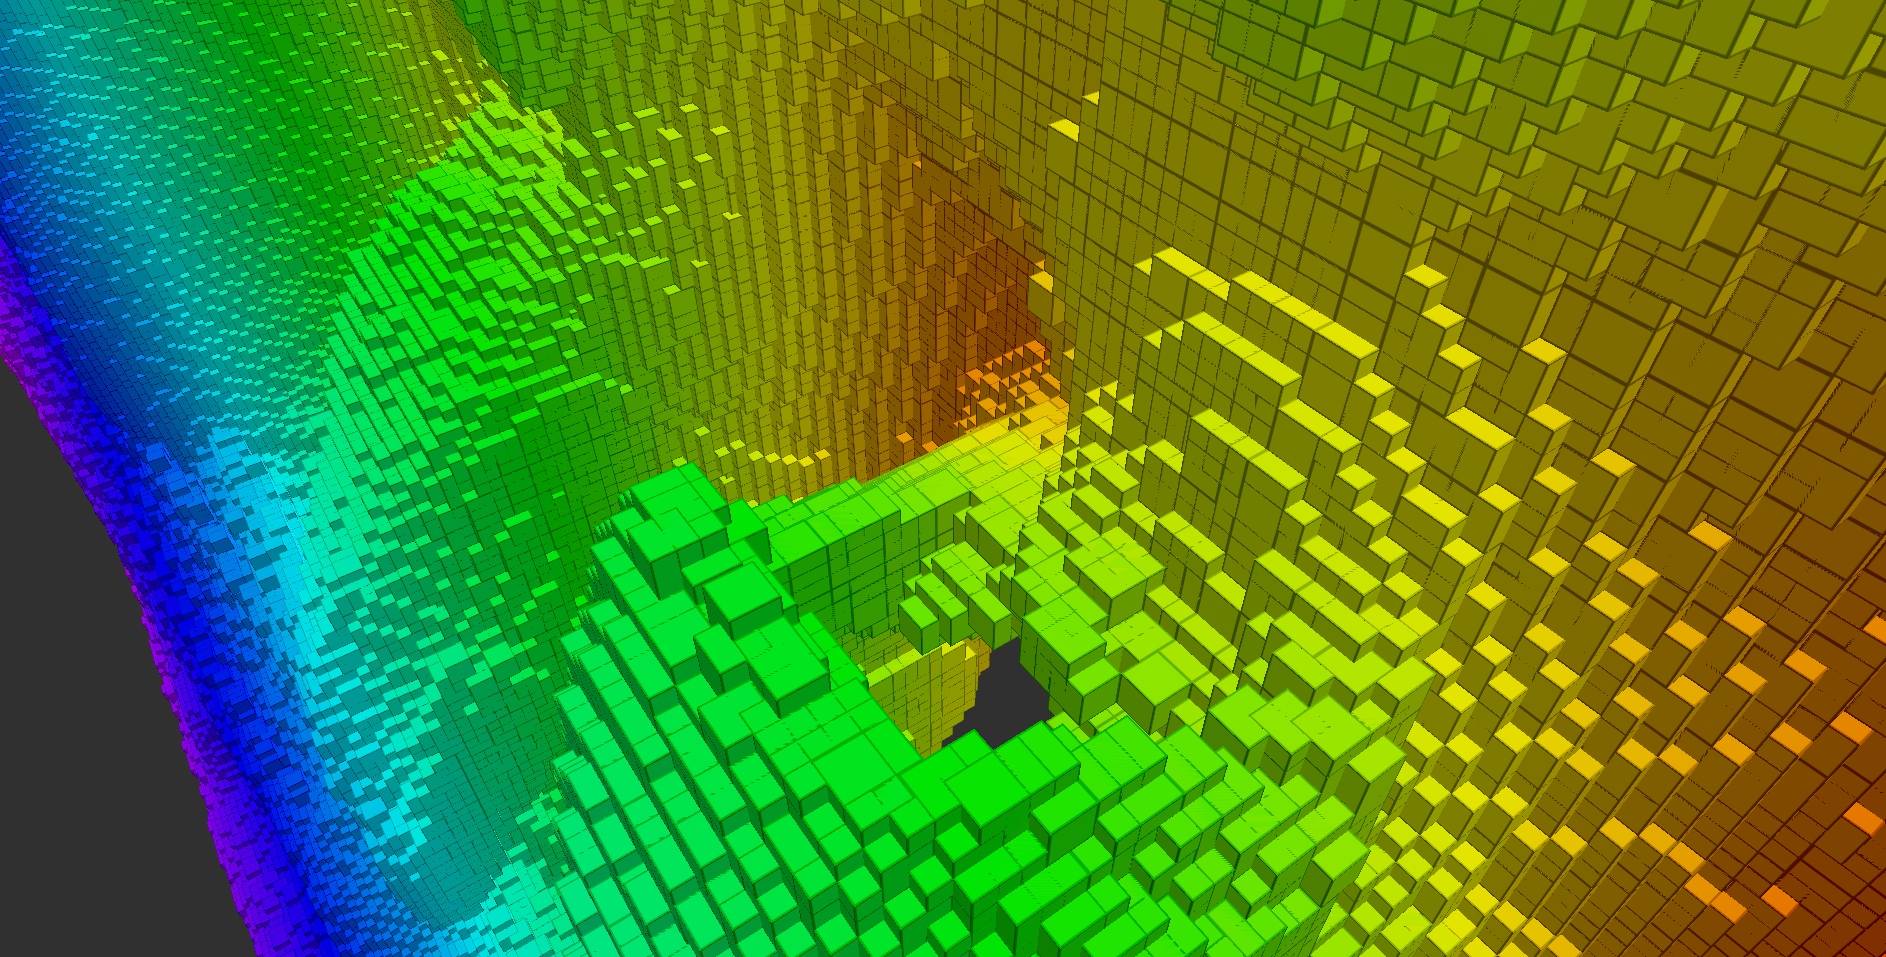
\includegraphics[width=0.23 \textwidth]{assets/FinalMappingHole1}
    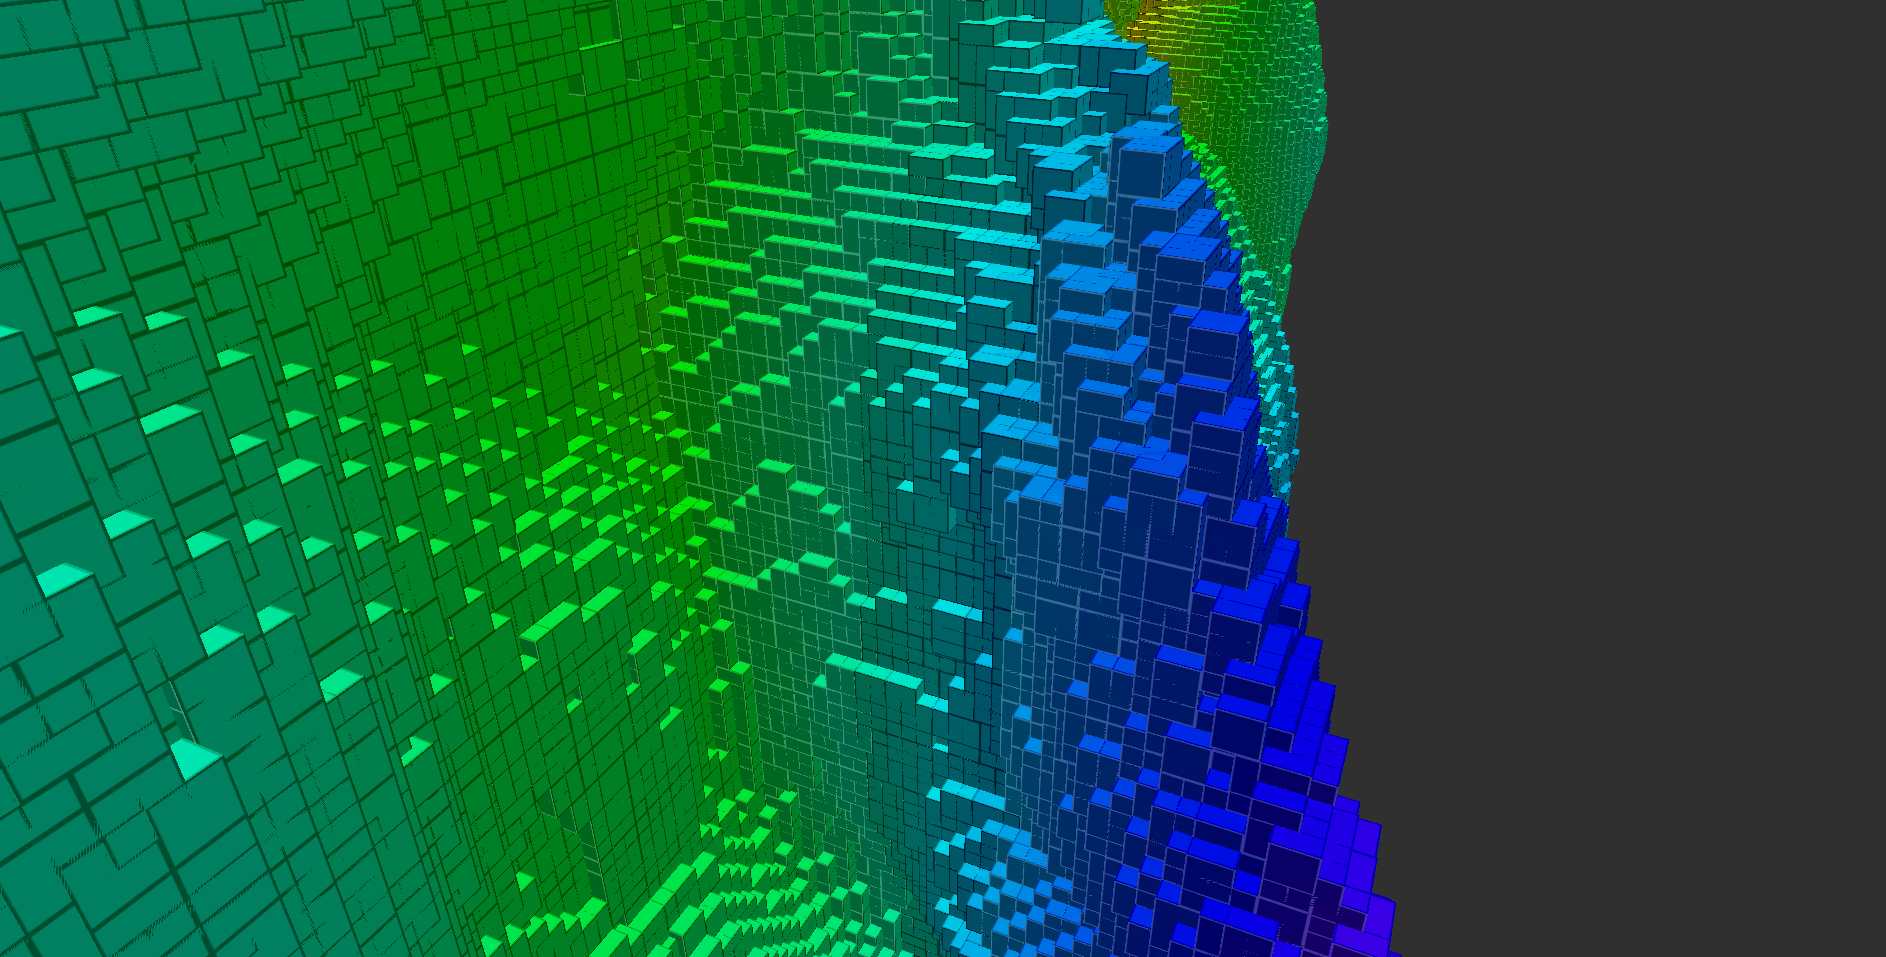
\includegraphics[width=0.23 \textwidth]{assets/FinalMappingHole2}
    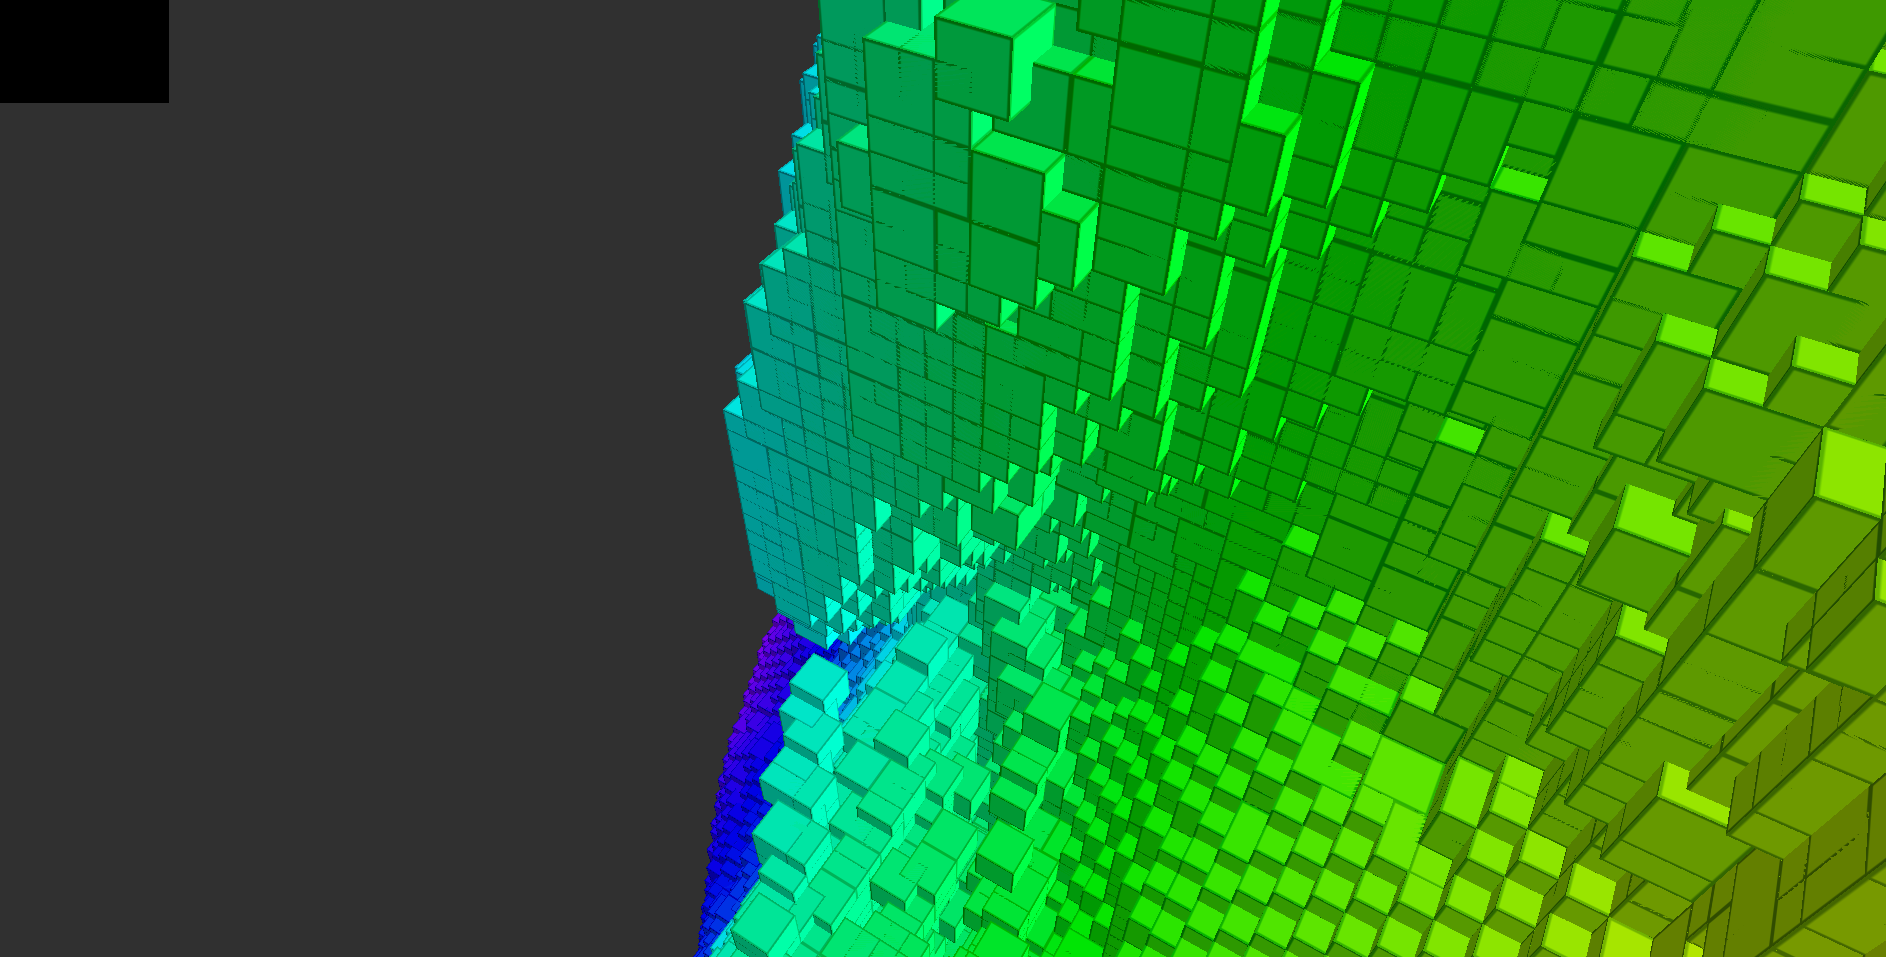
\includegraphics[width=0.23 \textwidth]{assets/FinalMappingHole3}
    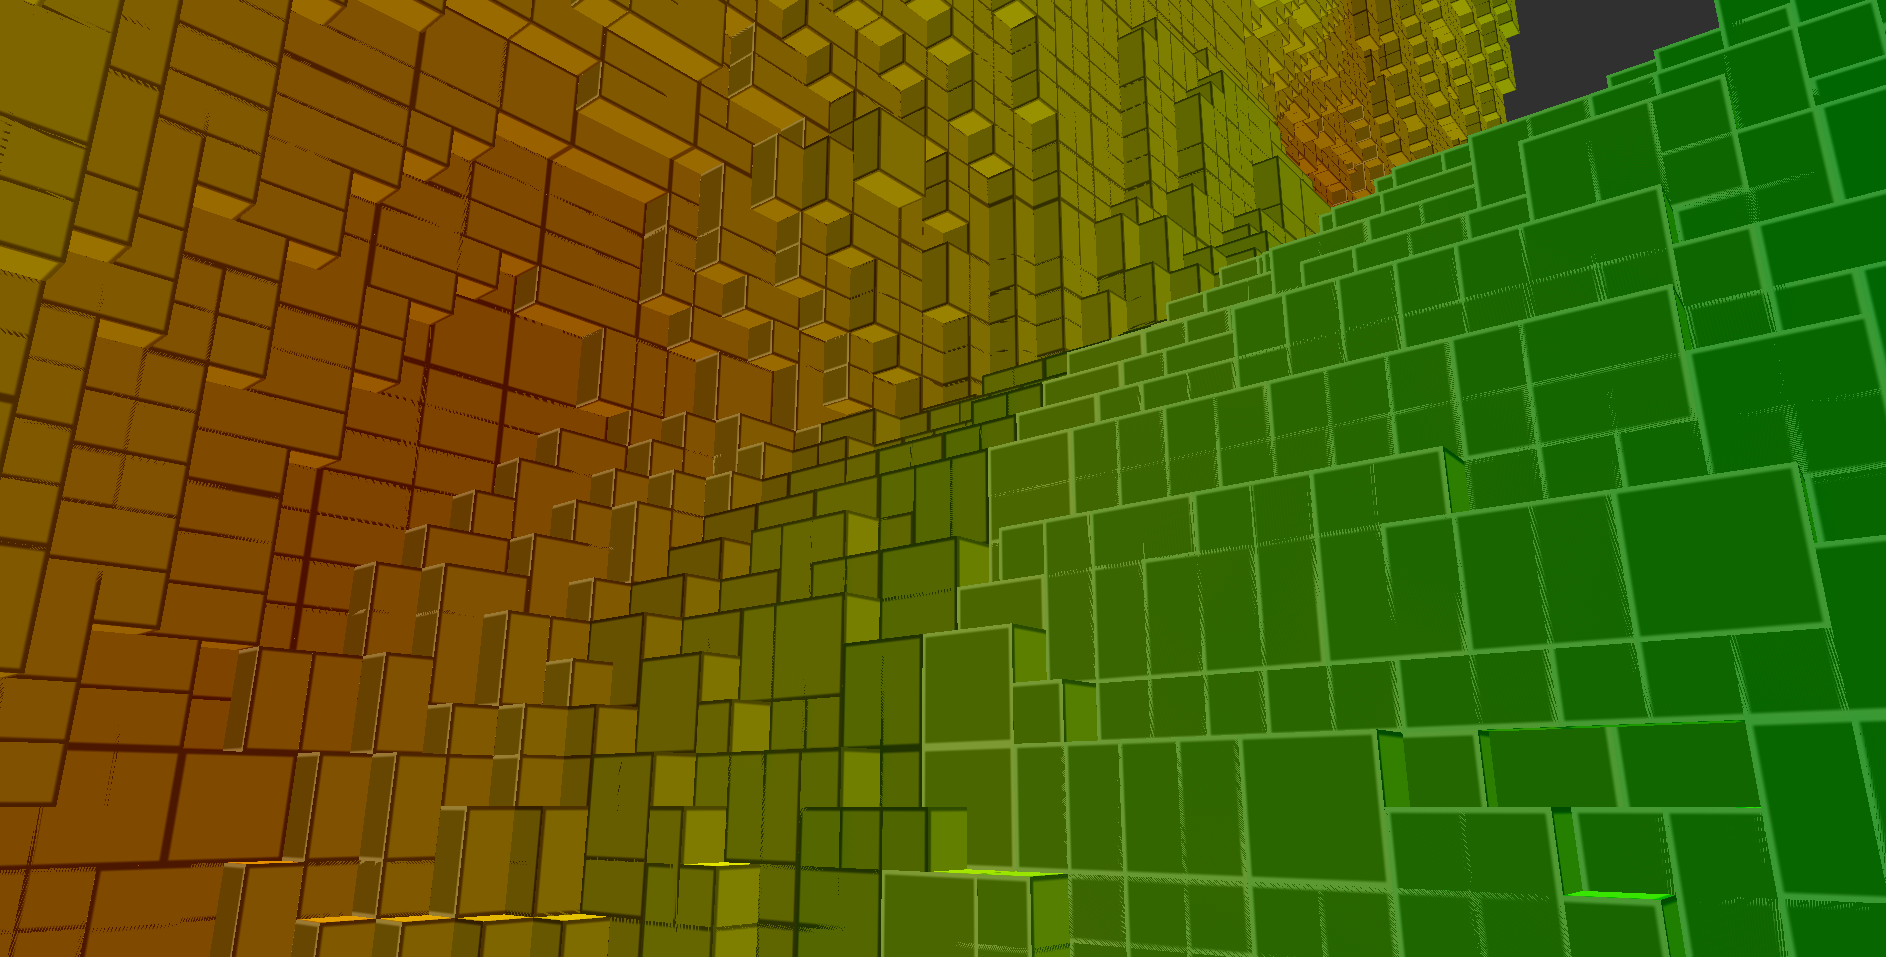
\includegraphics[width=0.23 \textwidth]{assets/FinalMappingHole4}
    }
  \end{center}
\vspace{-20pt}
  \caption{Mapping Problems using the Distance Algorithm with Rotation}
  \label{fig:secondMappingProblems}
\vspace{12pt}
\end{wrapfigure}

\begin{wrapfigure}{l}{\textwidth}
\vspace{-50pt}
\end{wrapfigure}

\section{Limitations and Possible Extensions}
\label{sec:limitations}
Due to time constraints, this paper is not extensive enough to cover all optimization possibilities. This section will therefore point out limitations of our algorithm and ideas on how to implement these.

\subsection{Obstacle avoidance}
Using the current algorithm, the robot might still run into some obstacles. If the robot for example navigates into a hole, it will not realize that it will crash into the ground. If there is something behind the robot and the robot tries to go backwards it will also not realize this. There exist different possible solutions for this problem. We could, for instance, add more sensors to the robot and use them to implement a behavior-based collision avoidance algorithm similar to our approach of keeping the distance to the reef. The advantage of this approach would be that it is easy to implement and we would additionally be able to react to dynamic objects in the environment like fish.\\

Since adding sensors would be cost intensive, we ideally have to move the robot's sensor or the robot itself to create more information about its surroundings. We could then query the OctoMap around it by casting rays in our movement direction and then check if we have information about the area in which we want to move. If we already have mapped the area in that direction, we can use a behavior-based approach to keep a distance to objects. If we have no information available, we can rotate our sensor or robot towards the direction of movement and obtain the necessary information. Afterwards we continue our algorithm and use a behavior-based approach to keep a distance to any newly scanned objects. A clear disadvantage of this is that dynamic objects like fish might confuse our robot.\\

\subsection{Map Creation}
Under the current algorithm our map creation procedure is not optimal. The robot, for example, rotates every few seconds to obtain more data, which costs us time and would cost a real world robot a considerable amount of energy. It would therefore be advisable to actually rotate only the sensor when possible and only rotate the whole robot we actually need to do so in order to obtain more information. The idea here is to create a list of unscanned and incomplete parts by querying the OctoMap. Afterwards we could take this set and calculate a good movement and rotation path for our robot so that it can scan those parts. Another way we can improve our map creation is to add more sensors to the robot. As before this approach is easy but relatively expensive.\\

\subsection{Movement}
The robot moves in a stair-like format. It, for example, moves backwards, down, backwards, down, etc. Ideally the robot should move in a seamless motion and use interpolation to combine the knowledge of having to move backwards and down. Moreover we also could include our obtained OctoMap to create a reference path along which we want to move. Another point to mention is that we disregard how an underwater robot would behave in real life. For a real life robot, the algorithm would need to be changed according to the limitations of the real world movement capabilities of the robot. \\

One prominent example for is apparent in our approach to moving mostly vertically instead of horizontally along the reef. Most underwater robots can move more effective horizontally and it is therefore a good idea to move sideways if possible. Nevertheless this could be implemented by simply changing some variables in our code.\\ 

\section{Conclusion}
\label{sec:conclusion}

In this research project, we were trying to create a mapping of a given underwater reef. Using a robot, we began with a very simple algorithm that explores a rectangle in a sequential fashion. In the next step we ensured that the robot would always keep a certain distance to the reef but also not be too far away from the reef.\\

At this point in time the created mapping was already very good but it contained a few holes which we tried to fix in the next step. Therefore we improved the calculation of the distance the robot has to keep to the reef by not using the robots whole field of vision to compute how far away it needs to be but rather by only using a smaller fraction of its vision, namely the part where the robot would move if it were to move forwards. Thus we ensured that the robot can get closer to the reef even if there are spikes or other structures around that would otherwise deter the robot from going closer.\\

Using this improved algorithm, the robot was indeed able to create a better mapping and close up one of the holes from the previous mapping while reducing the size of the holes in the other cases. These other cases were at spots on the side of elevated reef structures. To further improve our algorithm, we therefore added horizontal rotational movements to the algorithm in order to see the sides of the structures around us. This filled most of the remaining holes. The only hole that remained in the map is on the top of an elevated reef structure. To remove it, we would need to add vertical rotations as well.\\

Unfortunately, this research could not be tested in a real life scenario, and we can therefore not make any claims about its real-life performance. We strongly recommend creating a better algorithm for obstacle avoidance before testing this algorithm in a real life scenario. We also would suggest that we develop an algorithm to ensure that we only rotate the robot when absolutely necessary which then predominantly only rotates the sensors.\\

In conclusion, the created algorithm successfully creates a mapping of a reef structure. As pointed out in \autoref{sec:limitations}, there are some improvements that could be made to make the mapping even better. As is the mapping is already very good and almost complete. Depending on the requirements for the level of completeness of the mapping, this research might already be enough to give satisfactory results in a real-life scenario.\\

\newpage

\bibliography{kwarc}{}
\bibliographystyle{alpha}
\end{document}
